\documentclass{article}
%\usepackage{ctex}
\usepackage{amsmath}
\usepackage{amsfonts}

\usepackage{graphicx}                                                           
\usepackage{float}

\usepackage{listings}
\usepackage{xcolor}
\usepackage{booktabs}
\usepackage{algorithm}
%\usepackage{algorithmic}
\usepackage{algorithmicx} 
\usepackage{algpseudocode}

\definecolor{mygreen}{rgb}{0,0.6,0}
\definecolor{mygray}{rgb}{0.5,0.5,0.5}
\definecolor{mymauve}{rgb}{0.58,0,0.82}
\lstset{
 backgroundcolor=\color{lightgray}, 
 basicstyle = \footnotesize,       
 breakatwhitespace = false,        
 breaklines = true,                 
 captionpos = b,                    
 commentstyle = \color{mygreen}\bfseries,
 extendedchars = false,             
 frame =shadowbox, 
 framerule=0.5pt,
 keepspaces=true,
 keywordstyle=\color{blue}\bfseries, % keyword style
 language = C++,                     % the language of code
 otherkeywords={string}, 
 numbers=left, 
 numbersep=5pt,
 numberstyle=\tiny\color{mygray},
 rulecolor=\color{black},         
 showspaces=false,  
 showstringspaces=false, 
 showtabs=false,    
 stepnumber=1,         
 stringstyle=\color{mymauve},        % string literal style
 tabsize=2,          
 title=\lstname                      
}


\title{\textbf{Project Test Report}}
\author{Zhehao Chen 3220103172
  \thanks{Electronic address: \texttt{3220103172@zju.edu.cn}}}
\date{\today}

\begin{document}

\maketitle

\section*{Abstract}
This project report delves into the implementation and testing of piecewise polynomial splines in both the pp-Form and B-Form, focusing on their application in curve fitting and self-intersection detection. The study includes a comprehensive analysis of linear, quadratic, and cubic splines under various boundary conditions, such as natural, clamped, and periodic. The report presents a detailed methodology for generating curve points, calculating distances between line segments, and detecting self-intersections using a threshold-based approach.

\tableofcontents
\clearpage

\section{Test of pp-Form}

\subsection{Test Linear pp-Spline}
See \texttt{testLinearpp.cpp} for the test code.
\subsubsection{Methodology}
The interpolation was performed using the following steps:
\begin{enumerate}
    \item Define the function $f(x) = \sin(\pi x)$.
    \item Select a set of knots within the interval \([-1, 1]\).
    \item Compute the corresponding function values at these knots.
    \item Create a LinearSpline object with the knots and values.
\end{enumerate}

\subsubsection{Results}
The resulting plot of the linear spline interpolation is shown in Figure \ref{fig:spline_plot}. The plot displays the original data points and the linear spline that connects them.

\begin{figure}[H]
    \centering
    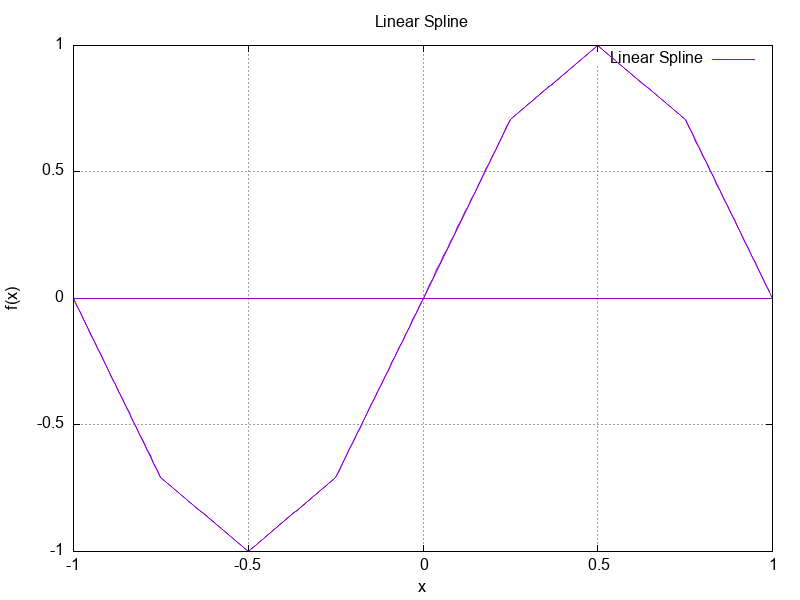
\includegraphics[width=0.4\textwidth]{../figure/Lppspline_plot.png}
    \caption{Linear Spline Interpolation of $f(x) = \sin(\pi x)$}
    \label{fig:spline_plot}
\end{figure}

\subsubsection{Discussion}
The plot in Figure \ref{fig:spline_plot} illustrates the linear segments that connect the data points. The spline appears to approximate the sine wave well within the given interval. However, the linear nature of the spline segments results in a piecewise linear curve that does not follow the smooth curvature of the sine function. This is an inherent limitation of linear spline interpolation when compared to higher-order splines or other interpolation methods.


\subsection{Test Cubic pp-Spline}
See \texttt{testCubicpp.cpp} for the test code.
\subsubsection{Methodology}
The interpolation was performed using the following steps:
\begin{enumerate}
    \item Define the sine function and generate knots within the interval \([-1, 1]\).
    \item Compute the function values at these knots.
    \item Create cubic splines with natural, clamped, and periodic boundary conditions.
\end{enumerate}

\subsubsection{Results}
The results of the cubic spline interpolation for the sine function with different boundary conditions are shown in Figures \ref{fig:natural}, \ref{fig:clamped}, and \ref{fig:periodic}. The plots display the spline and the knots for each boundary condition.

\begin{figure}[H]
    \centering
    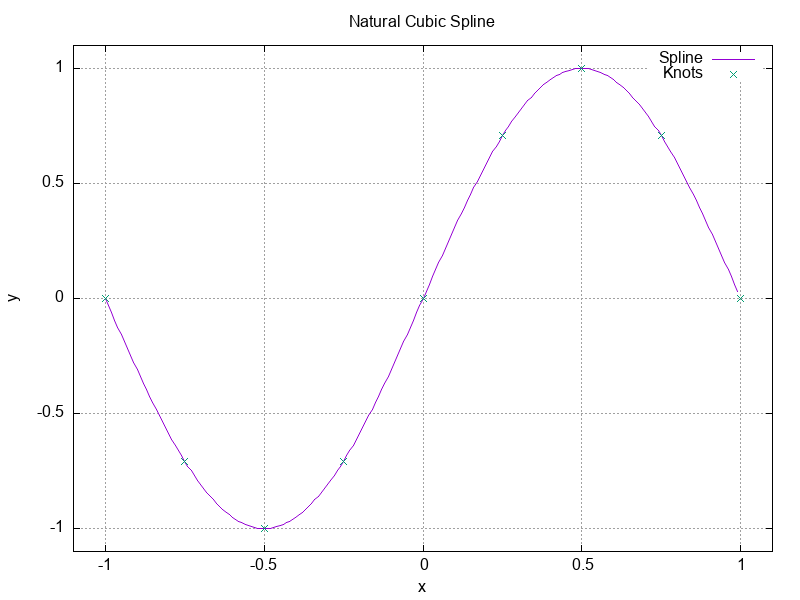
\includegraphics[width=0.5\textwidth]{../figure/Natural_spline_plot.png}
    \caption{Natural Boundary Condition Spline}
    \label{fig:natural}
\end{figure}

\begin{figure}[H]
    \centering
    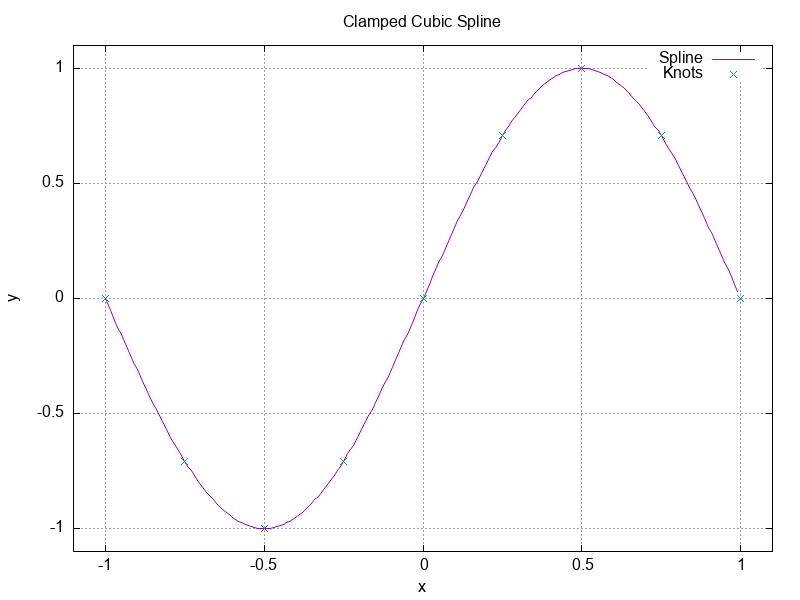
\includegraphics[width=0.5\textwidth]{../figure/Clamped_spline_plot.png}
    \caption{Clamped Boundary Condition Spline}
    \label{fig:clamped}
\end{figure}

\begin{figure}[H]
    \centering
    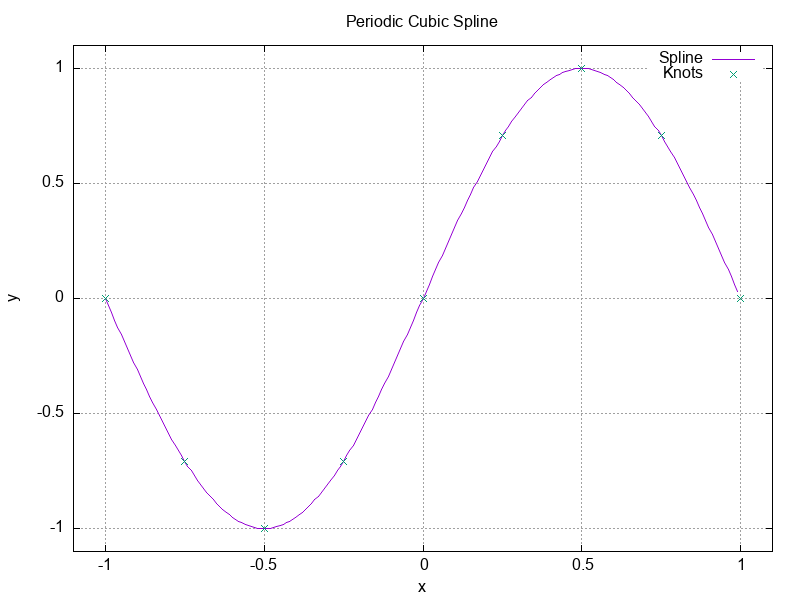
\includegraphics[width=0.5\textwidth]{../figure/Periodic_spline_plot.png}
    \caption{Periodic Boundary Condition Spline}
    \label{fig:periodic}
\end{figure}

\subsubsection{Answer of Problem A}
See \texttt{ProblemA.cpp} for the test code.\par
We solve the problem using the following steps:
\begin{enumerate}
    \item Define the function $f(x) = \frac{1}{1 + 25x^2}$.
    \item Generate evenly spaced nodes within the interval \([-1, 1]\).
    \item Compute the function values at these nodes.
    \item Create a CubicSpline (Natural Boundary Condition) object with natural boundary conditions.
    \item Calculate the maximum and mean squared errors for each node count.
\end{enumerate}
The results of the cubic spline interpolation for different node counts are shown in Figures \ref{fig:N6} to \ref{fig:N21}. The plots display the exact function and the interpolated spline, with the node count increasing from 6 to 81.

\begin{figure}[H]
    \centering
    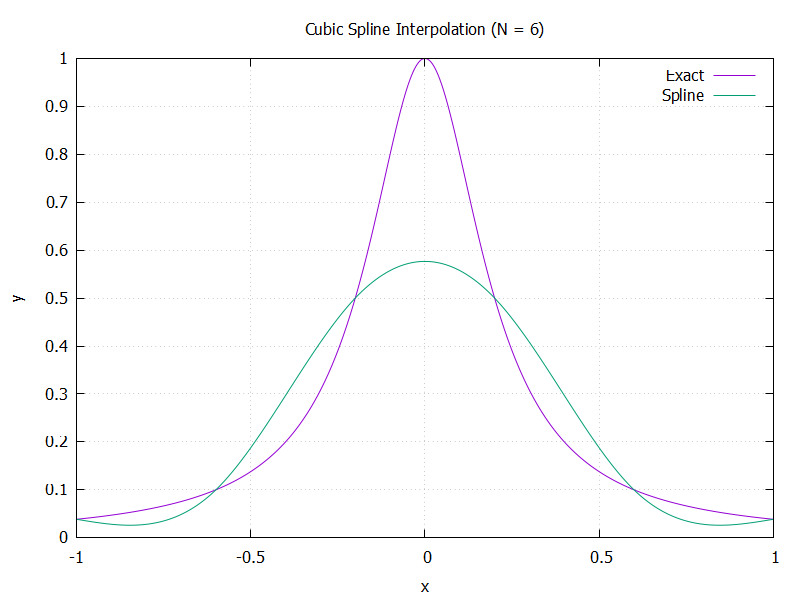
\includegraphics[width=0.45\textwidth]{../figure/cubic_spline_plot_N6.png}
    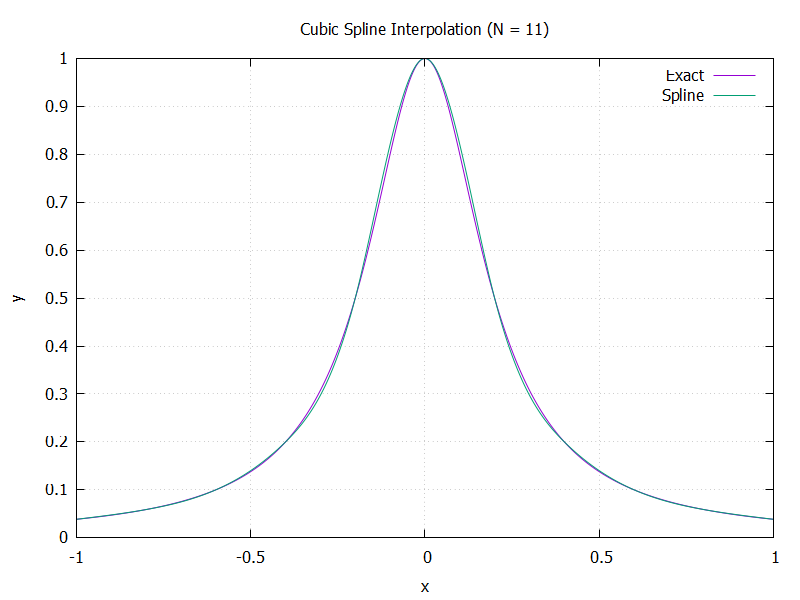
\includegraphics[width=0.45\textwidth]{../figure/cubic_spline_plot_N11.png}
    \caption{Cubic Spline Interpolation for N = 6 and N = 11}
    \label{fig:N6}
\end{figure}

\begin{figure}[H]
    \centering
    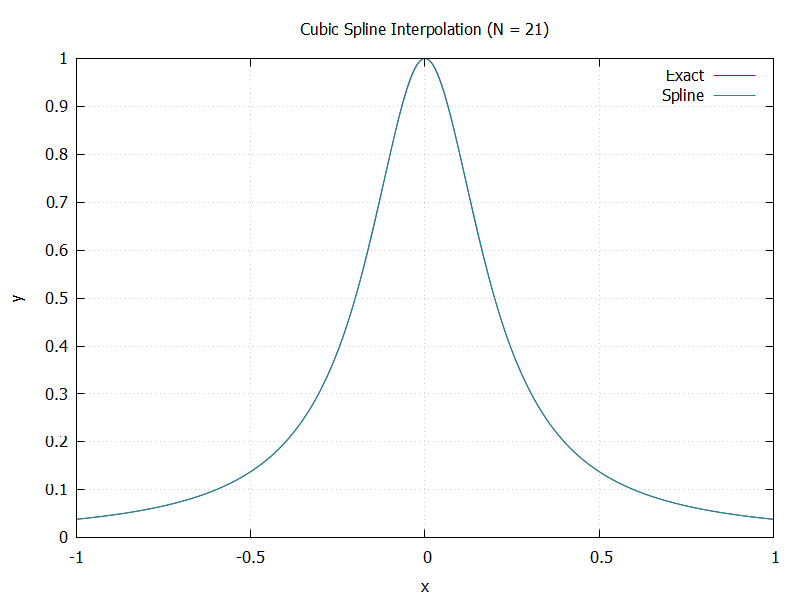
\includegraphics[width=0.45\textwidth]{../figure/cubic_spline_plot_N21.png}
    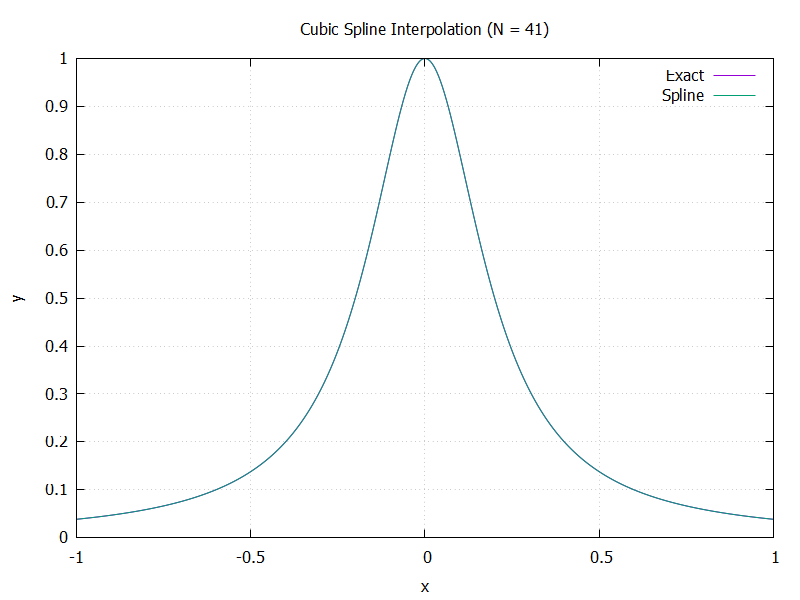
\includegraphics[width=0.45\textwidth]{../figure/cubic_spline_plot_N41.png}
    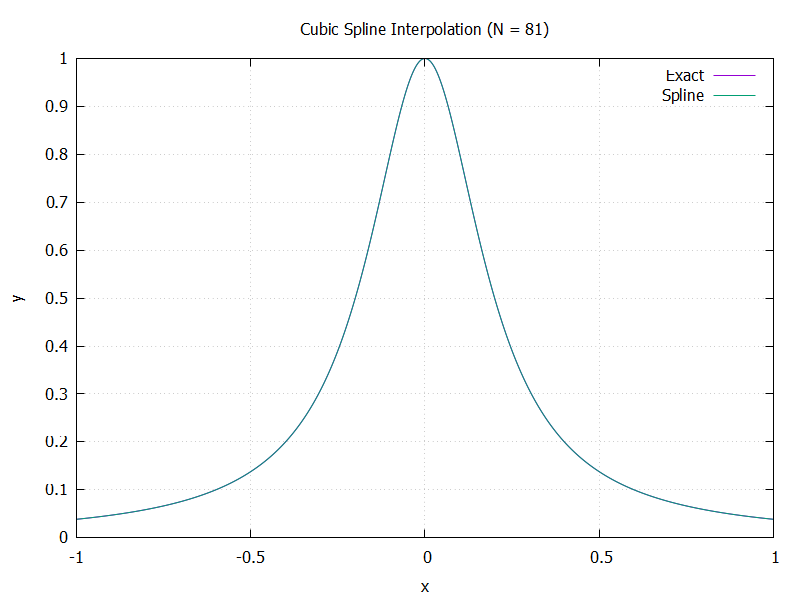
\includegraphics[width=0.45\textwidth]{../figure/cubic_spline_plot_N81.png}
    \caption{Cubic Spline Interpolation for N = 21, N = 41 and N = 81}
    \label{fig:N21}
\end{figure}

The error analysis results for different numbers of nodes are as follows:

\begin{table}[H]
\centering
\begin{tabular}{|c|c|c|}
\hline
Number of Nodes (N) & Maximum Error & Mean Squared Error \\ \hline
6 & 0.423389 & 0.0171987 \\ \hline
11 & 0.0219738 & 5.1134e-005 \\ \hline
21 & 0.00318131 & 7.71381e-007 \\ \hline
41 & 0.000277477 & 2.44319e-009 \\ \hline
81 & 1.58168e-005 & 5.56488e-012 \\ \hline
\end{tabular}
\caption{Error Analysis for Different Numbers of Nodes}
\label{tab:error_analysis}
\end{table}

\subsubsection{Discussion}
The plots illustrate the influence of boundary conditions on the spline interpolation:
\begin{itemize}
    \item Natural splines have zero second derivatives at the boundaries, resulting in a smooth curve with no overshoot.
    \item Clamped splines have specified first derivatives at the boundaries, which can lead to overshoots if the derivatives are large.
    \item Periodic splines are continuous and have the same slope at both ends, which is suitable for cyclic data.
\end{itemize}

\subsubsection{Conclusion}
The cubic spline interpolation of the sine function demonstrates how different boundary conditions can affect the interpolation result. Natural splines are smooth without overshoots, clamped splines can have overshoots due to specified derivatives, and periodic splines are ideal for cyclic data. The choice of boundary condition should be based on the specific requirements of the application.


\subsection{Test Degree 4 pp-Spline}
See \texttt{testD4pp.cpp} for the test code.
\subsubsection{Methodology}
\begin{enumerate}
    \item Generation of evenly spaced nodes within the interval \([-1, 1]\).
    \item Calculation of function values at these nodes using the function \( f(x) = \frac{1}{1 + 25x^2} \).
    \item Construction of a Degree-4 spline using these nodes and function values.
    \item Evaluation of the spline at a finer set of points to compare with the exact function values.
    \item Calculation of interpolation errors.
    \item Generation of a plot using Gnuplot to visualize the exact function and the spline interpolation.
\end{enumerate}

\subsubsection{Results}
The test generated a plot comparing the exact function and the Degree-4 spline interpolation, as shown in Figure \ref{fig:spline_plot}. The plot illustrates the spline's ability to closely approximate the exact function over the interval.

\begin{figure}[H]
    \centering
    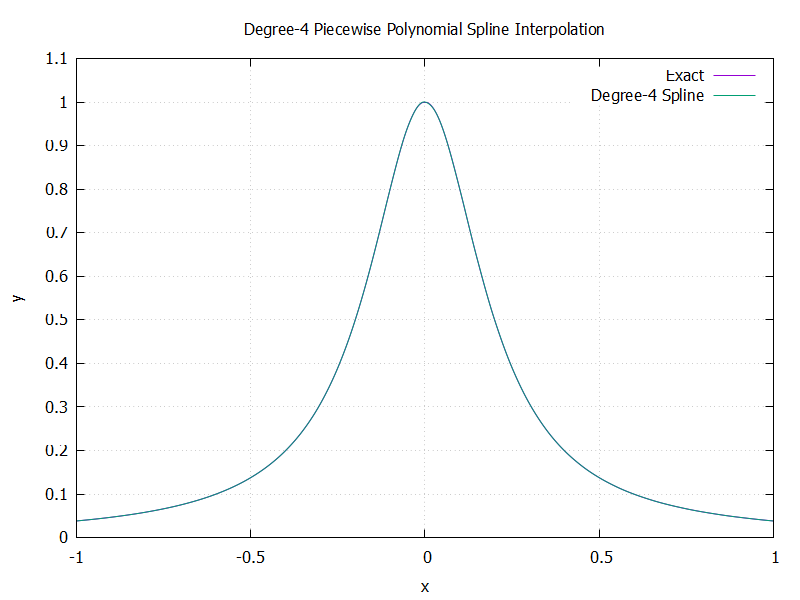
\includegraphics[width=0.8\textwidth]{../figure/degree4_spline_plot.png}
    \caption{Comparison of the exact function and the Degree-4 spline interpolation.}
    \label{fig:spline_plot}
\end{figure}

The test also calculated the maximum error and the mean squared error for the interpolation, providing quantitative measures of the spline's accuracy.

\subsubsection{Discussion}
The results indicate that the Degree-4 spline provides a good approximation of the exact function, with the plot showing a close match between the spline and the exact function curve.


\subsection{Test Degree 5 pp-Spline}
See \texttt{testD5pp.cpp} for the test code.
\subsubsection{Methodology}
Most of the steps are the same as "Test Degree 5 pp-Spline", except:
\begin{enumerate}
    \item Generation of evenly spaced nodes within the interval \([-3, 3]\).
    \item Calculation of function values at these nodes using the function \( f(x) = \frac{1}{e^{x^2}} \).
\end{enumerate}

\subsubsection{Results}
The spline interpolation was performed with 11 nodes, and the results are visualized in the provided plot. The plot shows a close match between the exact function and the interpolated spline, indicating the effectiveness of the interpolation method.

\begin{figure}[H]
    \centering
    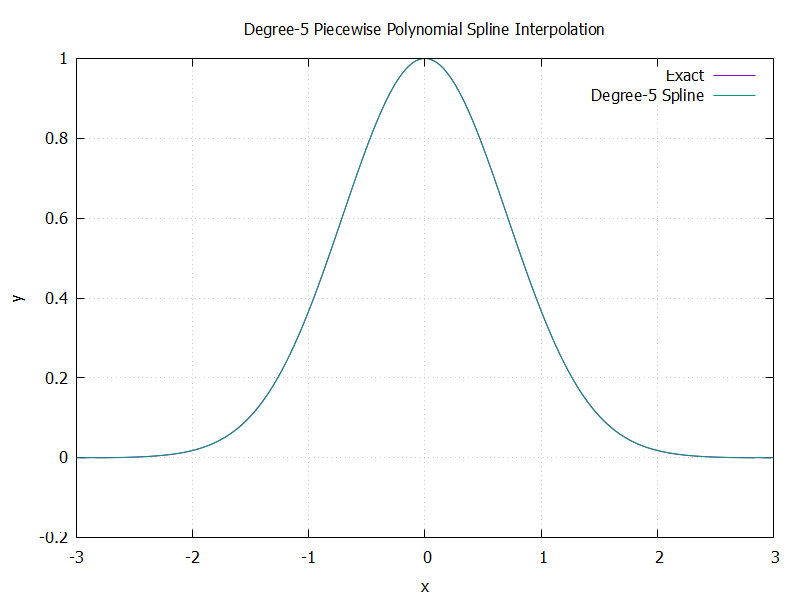
\includegraphics[width=\textwidth]{../figure/degree5_spline_plot.png}
    \caption{Degree-5 Piecewise Polynomial Spline Interpolation of \( f(x) = \frac{1}{e^{x^2}} \)}
    \label{fig:degree5_spline}
\end{figure}

\subsubsection{Discussion}
The results demonstrate that the degree-5 spline provides a good approximation of the function within the given interval. The plot visually confirms the spline's ability to capture the general shape and behavior of the function, with minor deviations from the exact curve.

\subsection{Test Curve-fitting of pp-Form}
See \texttt{ppheartCurve.cpp} for the test code.
\subsubsection{Methodology}
The interpolation was performed using the following steps:
\begin{enumerate}
    \item Define the heart curve parameters and generate t parameter points.
    \item Calculate the x and y points for the heart curve.
    \item Create cubic splines for x(t) and y(t) with different boundary conditions (natural, clamped, periodic).
    \item Generate Gnuplot scripts to plot the heart curve with each boundary condition.
    \item Run the Gnuplot scripts to produce the plots.
\end{enumerate}

\subsubsection{Results}
The results of the cubic spline interpolation for the heart curve with different boundary conditions are shown in Figures \ref{fig:natural}, \ref{fig:clamped}, and \ref{fig:periodic}. The plots display the heart curve with 10, 40, and 160 points for each boundary condition.

\begin{figure}[H]
    \centering
    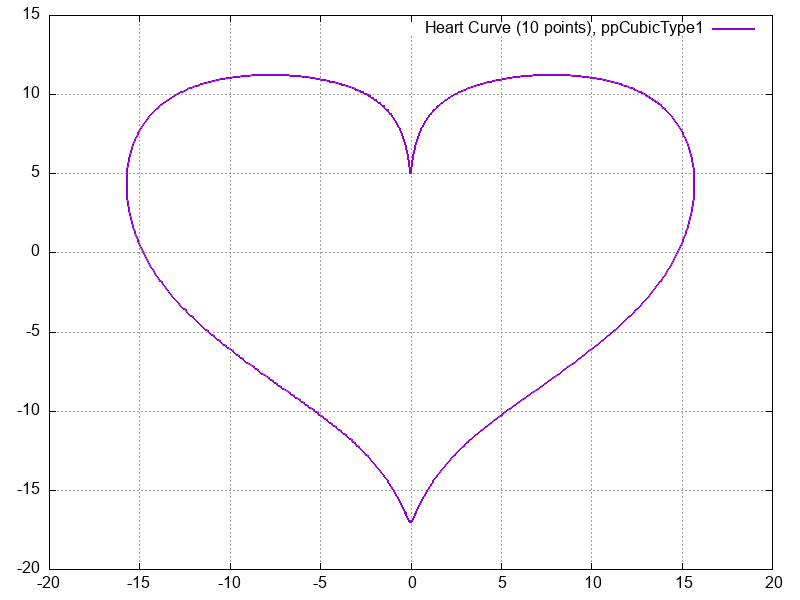
\includegraphics[width=0.45\textwidth]{../figure/pp1spline_plot_10.png}
    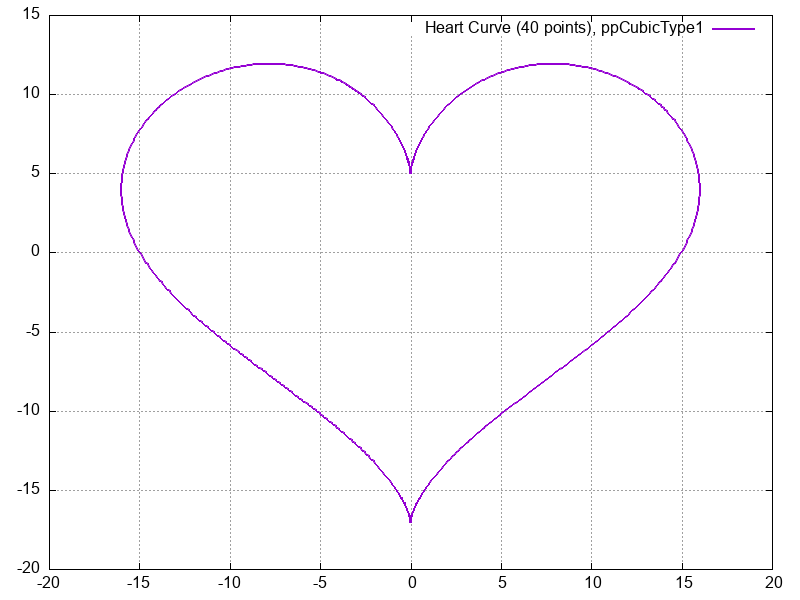
\includegraphics[width=0.45\textwidth]{../figure/pp1spline_plot_40.png}
    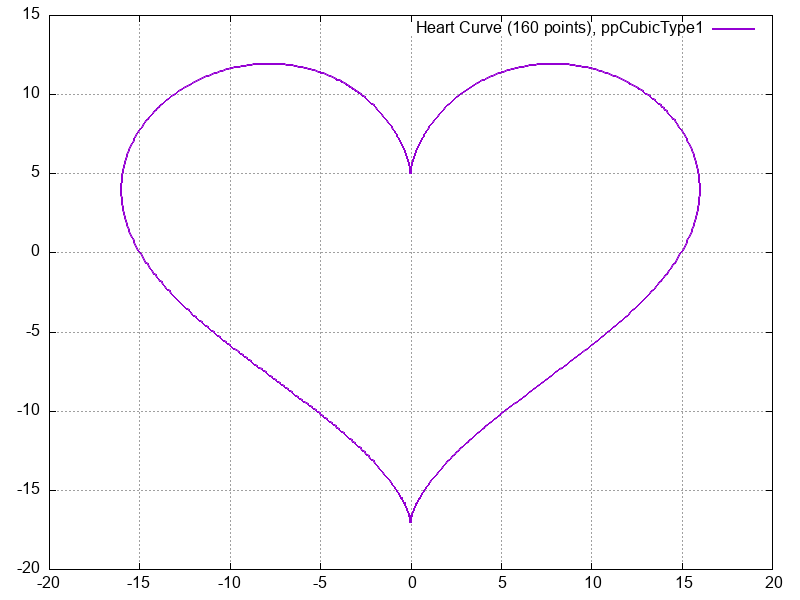
\includegraphics[width=0.45\textwidth]{../figure/pp1spline_plot_160.png}
    \caption{Heart Curve with Natural Boundary: Conditions (1)}
    \label{fig:natural}
\end{figure}

\begin{figure}[H]
    \centering
    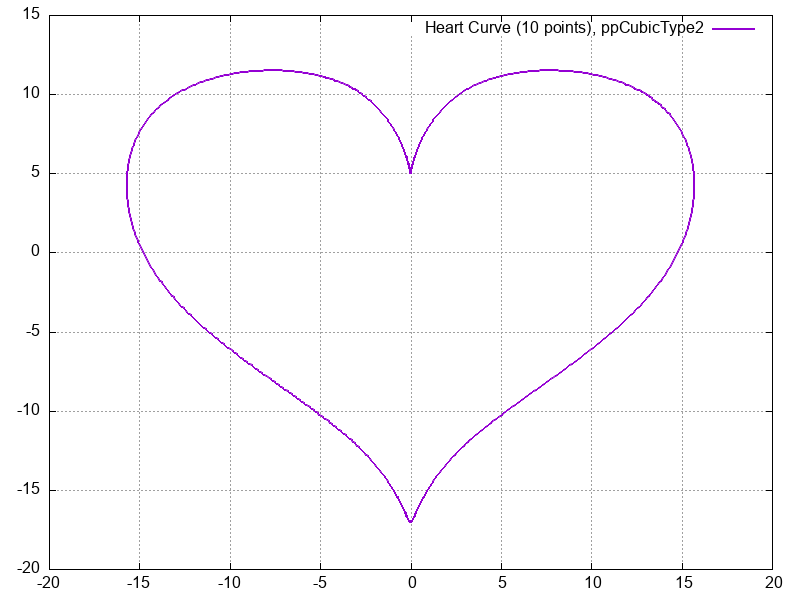
\includegraphics[width=0.45\textwidth]{../figure/pp2spline_plot_10.png}
    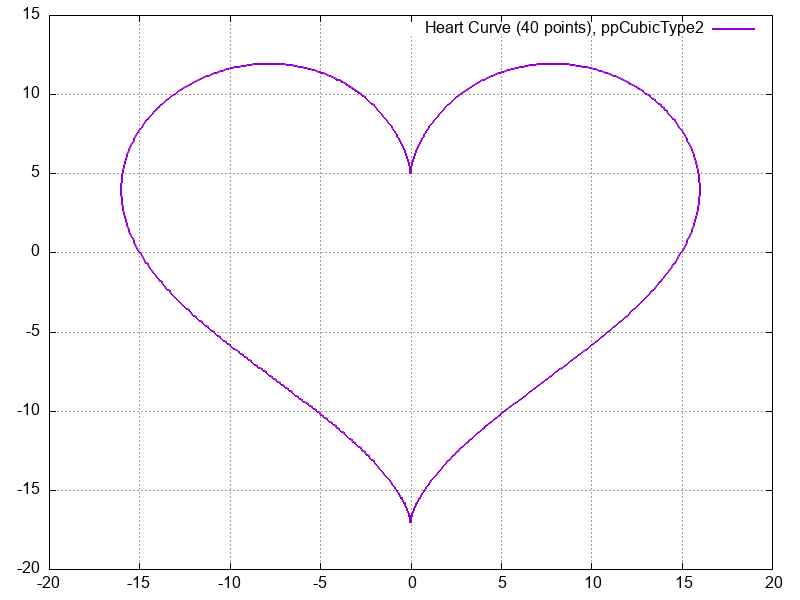
\includegraphics[width=0.45\textwidth]{../figure/pp2spline_plot_40.png}
    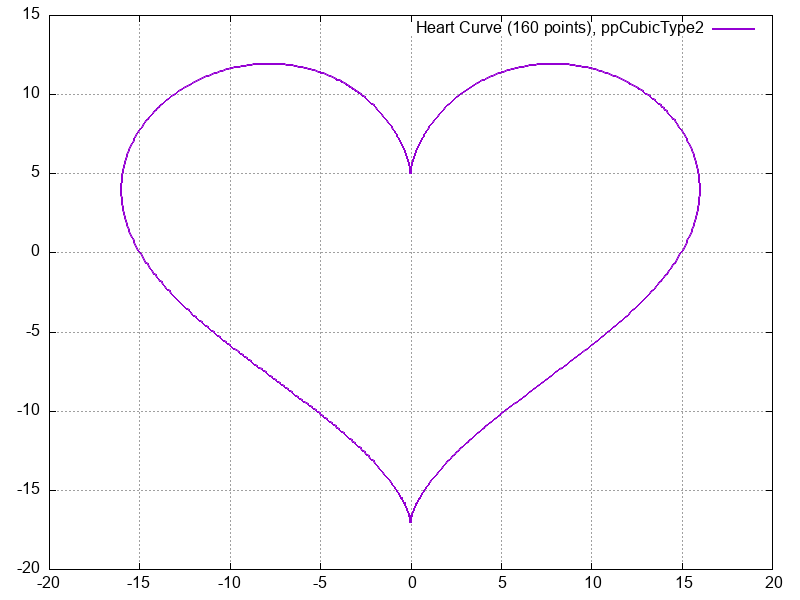
\includegraphics[width=0.45\textwidth]{../figure/pp2spline_plot_160.png}
    \caption{Heart Curve with Clamped Boundary: Conditions (2)}
    \label{fig:clamped}
\end{figure}

\begin{figure}[H]
    \centering
    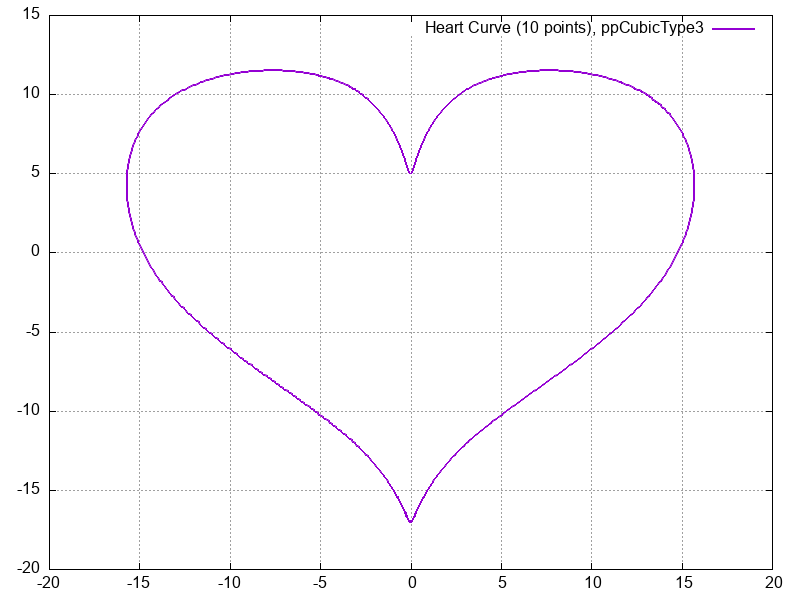
\includegraphics[width=0.45\textwidth]{../figure/pp3spline_plot_10.png}
    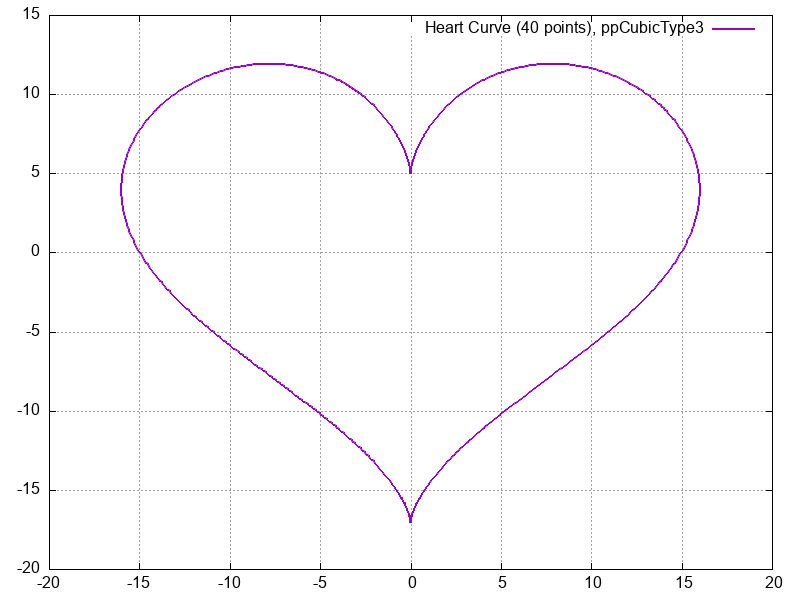
\includegraphics[width=0.45\textwidth]{../figure/pp3spline_plot_40.png}
    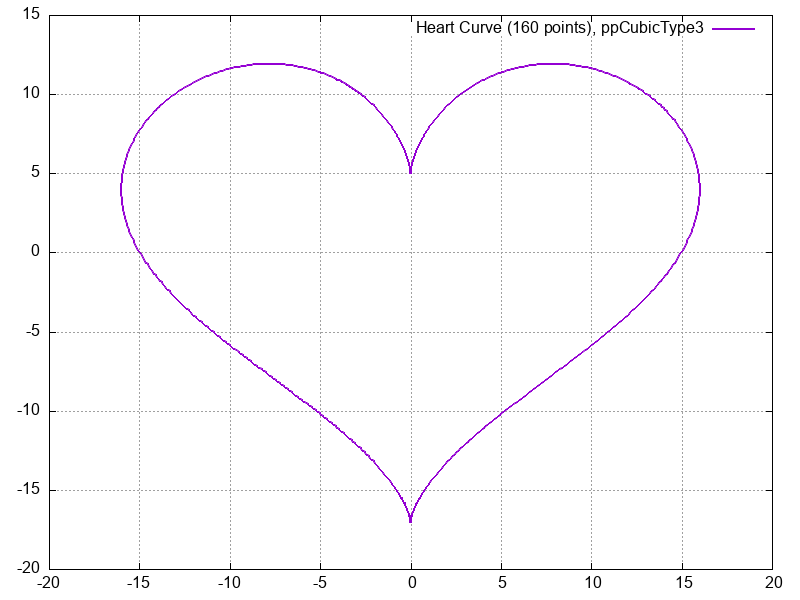
\includegraphics[width=0.45\textwidth]{../figure/pp3spline_plot_160.png}
    \caption{Heart Curve with Periodic Boundary: Conditions (3)}
    \label{fig:periodic}
\end{figure}

\subsubsection{Conclusion}
The cubic spline interpolation of the heart curve with different boundary conditions provides a visual demonstration of how boundary conditions influence the interpolation result. For applications requiring different types of boundary behavior, the appropriate cubic spline boundary condition can be selected to achieve the desired curve characteristics.


\section{Test of B-Form}
\subsection{Test Linear B-Spline}
See \texttt{testLinearB.cpp} for the test code.
\subsubsection{Methodology}
The interpolation was performed using the following steps:
\begin{enumerate}
    \item Define the function \( f(x) = \frac{1}{1 + x^2} \).
    \item Select a set of knots within the interval \([-5, 5]\).
    \item Compute the function values at these knots.
    \item Create a LinearBSpline object with the knots and values.
\end{enumerate}

\subsubsection{Results}
The result of the linear B-spline interpolation is shown in Figure \ref{fig:bspline}. The plot displays the original function and the interpolated B-spline.

\begin{figure}[h]
    \centering
    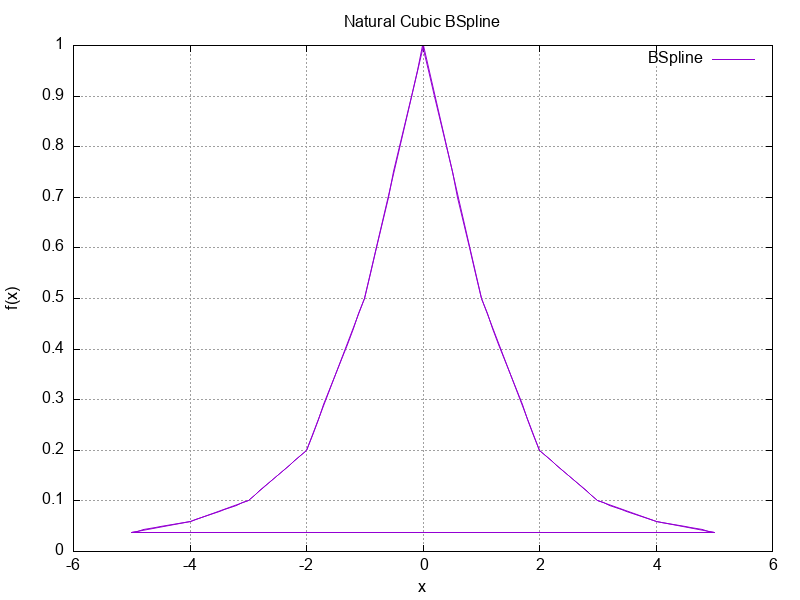
\includegraphics[width=0.5\textwidth]{../figure/LBspline_plot.png}
    \caption{Linear B-Spline Interpolation}
    \label{fig:bspline}
\end{figure}

\subsubsection{Discussion}
The plot in Figure \ref{fig:bspline} illustrates the linear B-spline interpolation of the function. The B-spline closely follows the shape of the original function, demonstrating the effectiveness of this interpolation method. Linear B-splines provide a straightforward and effective way to approximate raw data, suitable for occasions where high-order polynomial interpolation is not required.


\subsection{Test Quadratic B-Spline (Problem B\&C)}
See \texttt{testQuadraticB.cpp} for the test code.
\subsubsection{Methodology}
The interpolation was performed using the following steps:
\begin{enumerate}
    \item Define the function \( f(x) = \frac{1}{1 + x^2} \).
    \item Select a set of points within the interval \([-5, 5]\).
    \item Compute the function values at these points.
    \item Create a QuadraticBSpline object with the points and values.
\end{enumerate}

\subsubsection{Results}
The result of the quadratic B-spline interpolation is shown in Figure \ref{fig:qbspline}. The plot displays the original function and the interpolated B-spline.

\begin{figure}[H]
    \centering
    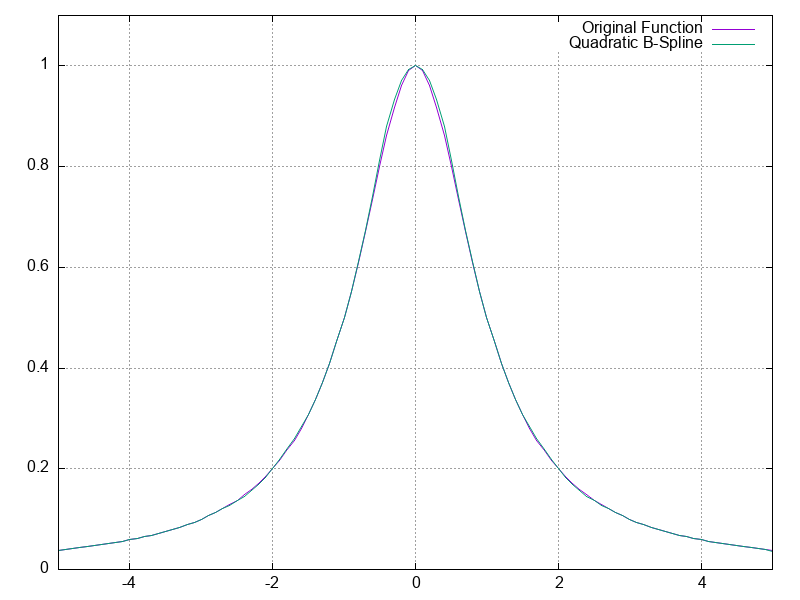
\includegraphics[width=0.8\textwidth]{../figure/QBspline_plot.png}
    \caption{Quadratic B-Spline Interpolation}
    \label{fig:qbspline}
\end{figure}

\subsubsection{Discussion}
The plot in Figure \ref{fig:qbspline} illustrates the quadratic B-spline interpolation of the function. The B-spline closely follows the shape of the original function, demonstrating the effectiveness of this interpolation method. Quadratic B-splines provide a smooth transition between data points and are particularly useful for their simplicity and efficiency.


\subsection{Test Cubic B-Spline (Problem B\&C)}
See \texttt{testCubicB.cpp} for the test code.
\subsubsection{Methodology}
The interpolation was performed using the following steps:
\begin{enumerate}
    \item Define the functions \( f_1(x) = \frac{1}{1 + x^2} \) (for Natural and Clamped) and \( f_2(x) = \sin(\pi x) \) (for Periodic).
    \item Select a set of nodes for each function.
    \item Compute the function values at these nodes.
    \item Create cubic B-spline objects with natural, clamped, and periodic boundary conditions.
\end{enumerate}

\subsubsection{Results}
The results of the cubic B-spline interpolation under different boundary conditions are shown in Figures \ref{fig:natural} and \ref{fig:periodic}. The plots display the original functions and the interpolated B-splines.

\begin{figure}[H]
    \centering
    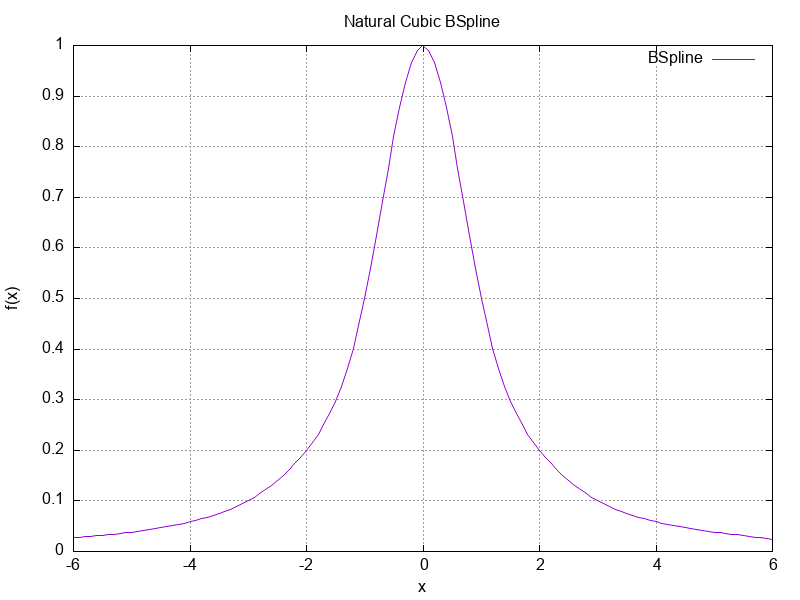
\includegraphics[width=0.45\textwidth]{../figure/NCBspline_plot.png}
    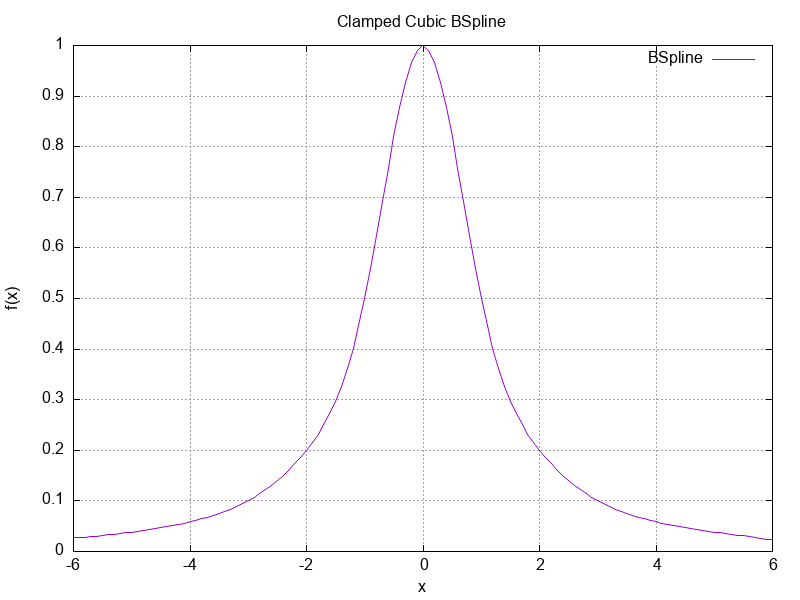
\includegraphics[width=0.45\textwidth]{../figure/CCBspline_plot.png}
    \caption{Natural and Clamped Cubic B-Spline Interpolation for \( f_1(x) \)}
    \label{fig:natural}
\end{figure}

\begin{figure}[H]
    \centering
    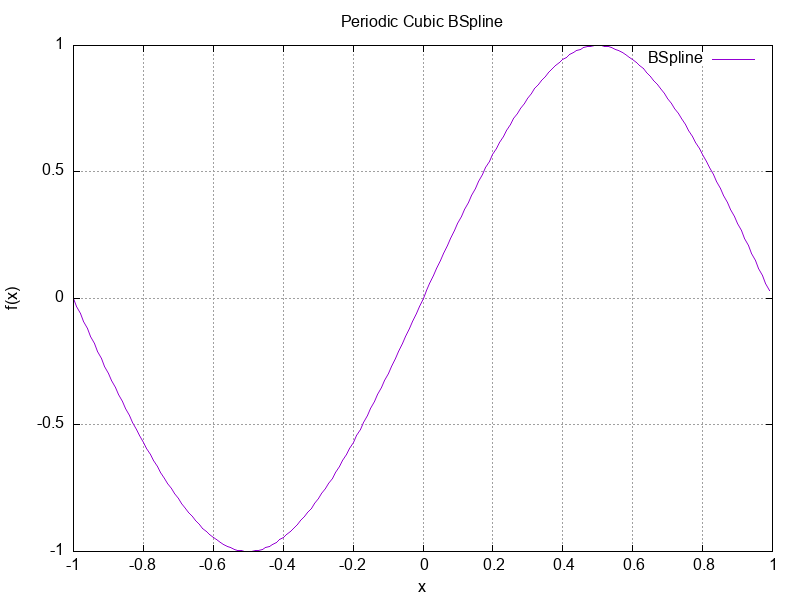
\includegraphics[width=0.5\textwidth]{../figure/PCBspline_plot.png}
    \caption{Periodic Cubic B-Spline Interpolation for \( f_2(x) \)}
    \label{fig:periodic}
\end{figure}

\subsubsection{Discussion}
The plots illustrate the influence of boundary conditions on cubic B-spline interpolation:
\begin{itemize}
    \item Natural splines have zero second derivatives at the boundaries, resulting in a smooth curve with no overshoot.
    \item Clamped splines have specified first derivatives at the boundaries, which can lead to overshoots if the derivatives are large.
    \item Periodic splines are continuous and have the same slope at both ends, which is suitable for cyclic data.
\end{itemize}


\subsection{Problem D}
See \texttt{ProblemD.cpp} for the test code.
\subsubsection{Methodology}
The interpolation was performed using the following steps:
\begin{enumerate}
    \item Define the function \( f(x) = \frac{1}{1 + x^2} \).
    \item Select a set of nodes within the interval \([-5, 5]\).
    \item Compute the function values at these nodes.
    \item Create quadratic and natural cubic B-spline objects.
\end{enumerate}

\subsubsection{Results}
The results of the quadratic and natural cubic B-spline interpolation are shown in Figures \ref{fig:bspline} and \ref{fig:error}. The plots display the original function, the quadratic B-spline, and the natural cubic B-spline. \par
\emph{Because we made the "midpoint" of the nodes in the implementation process so that the number of nodes and the number of function values are the same in the final operation to simplify the calculation, the error here may be different from the requirements in the book.}

\begin{figure}[H]
    \centering
    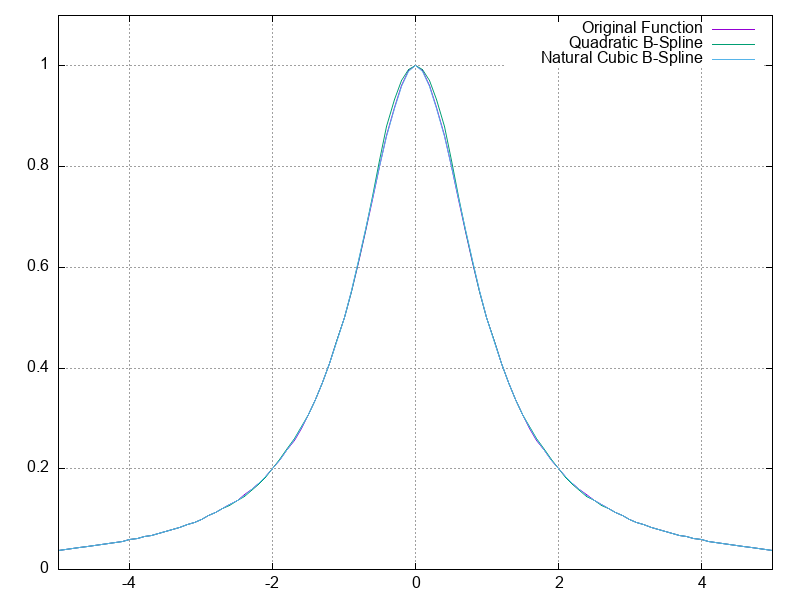
\includegraphics[width=0.8\textwidth]{../figure/QCBspline_plot.png}
    \caption{Quadratic and Natural Cubic B-Spline Interpolation}
    \label{fig:bspline}
\end{figure}

\begin{figure}[H]
    \centering
    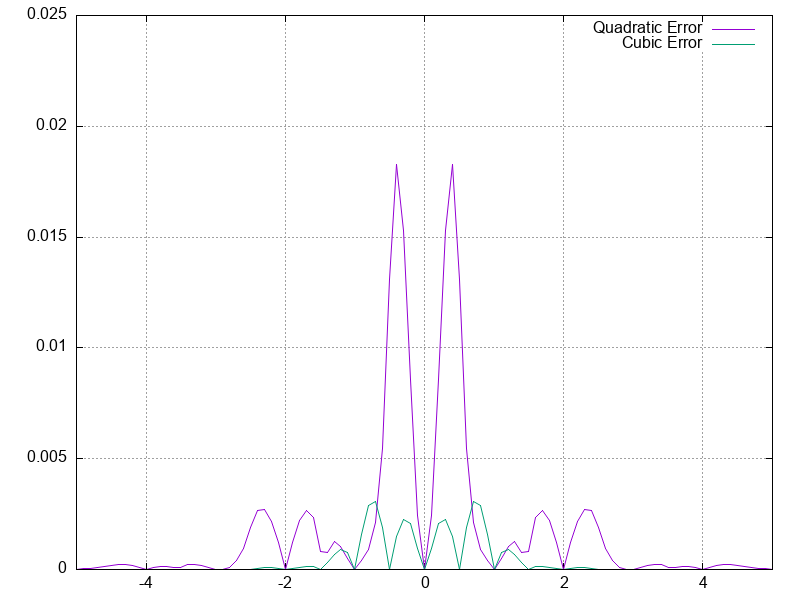
\includegraphics[width=0.8\textwidth]{../figure/error_plot.png}
    \caption{Interpolation Error for Quadratic and Cubic B-Splines}
    \label{fig:error}
\end{figure}

\begin{table}[H]
\centering
\caption{Error Analysis for Different Numbers of Nodes}
\label{tab:error_analysis}
\begin{tabular}{|c|c|c|}
\hline
\textbf{Site} & \textbf{Quadratic Error} & \textbf{Cubic Error} \\
\hline
-3.5 & $7.10258 \times 10^{-5}$ & $2.87991 \times 10^{-18}$ \\ \hline
-3   & $3.33053 \times 10^{-17}$ & $8.32803 \times 10^{-18}$ \\ \hline
-0.5 & 0.0130736 & $2.88669 \times 10^{-16}$ \\ \hline
0    & $1.11022 \times 10^{-16}$ & $1.11022 \times 10^{-16}$ \\ \hline
0.5  & 0.0130736 & $4.43981 \times 10^{-17}$ \\ \hline
3    & $8.32803 \times 10^{-18}$ & $5.54976 \times 10^{-18}$ \\ \hline
3.5  & $7.10258 \times 10^{-5}$ & $1.09979 \times 10^{-17}$ \\
\hline
\end{tabular}
\end{table}

\subsubsection{Discussion}
The plots in Figure \ref{fig:error} illustrate the interpolation error for both the quadratic and natural cubic B-splines. The errors close to machine precision are likely due to the high accuracy of the B-spline interpolation at the nodes and the smoothness of the B-spline curves. The cubic B-spline appears to be more accurate overall, as indicated by the smaller error values across the range.


\subsection{Any Order and Any Node Splines}
See \texttt{calculateBSpline.cpp} for the test code.\par
The B-Spline format should support the drawing of any order and any node splines. That is, to implement the formula:

\[
S(t) = \sum_{i=2-n}^{N} a_i B_i^n(t) \in \mathbb{S}_n^{n-1}(t_1, \ldots, t_N), \quad t \in [t_1, t_N]
\]
\subsubsection{Methodology}
The interpolation was performed using the following steps:
\begin{enumerate}
    \item The degree of the B-spline \( n \) was set to 4.
    \item The number of knots \( M \) was determined to be 20.
    \item Knot values were input in non-decreasing order: 1, 2, 3, 5, 9, 10, 11, 12, 15, 16, 18, 19, 21, 22, 24, 30, 31, 32, 35, 37, (At the beginning and end, you are required to enter additional nodes that do not draw curves).
    \item Control point coefficients were input for the B-spline: 8, 5, 9, 14, 5, 6, 3, 2, 1, 4, 16, 9, 21, 11, 10.
\end{enumerate}

\subsubsection{Results}
The result of the B-spline interpolation is shown in Figure \ref{fig:bspline}. The plot displays the B-spline curve generated from the input parameters.

\begin{figure}[H]
    \centering
    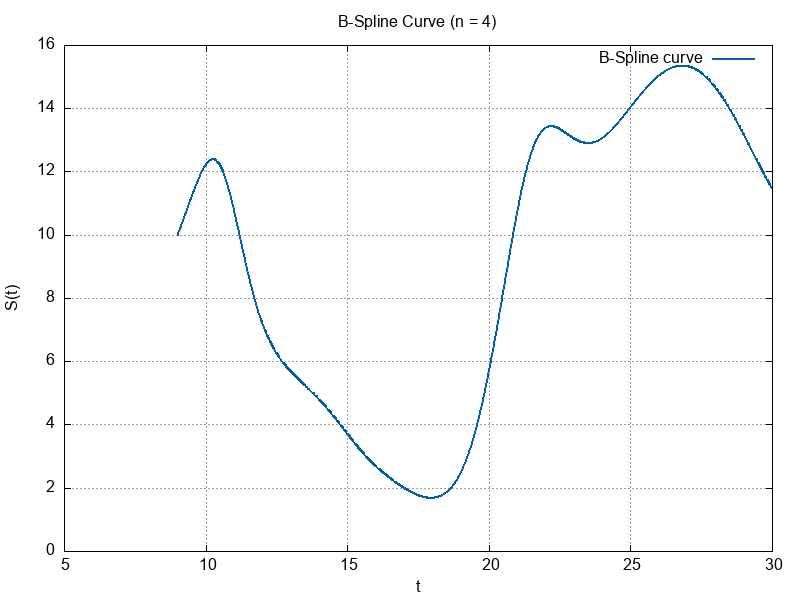
\includegraphics[width=\textwidth]{../figure/n_degree_BSpline_plot.png}
    \caption{B-Spline Curve (n = 4)}
    \label{fig:bspline}
\end{figure}

\subsubsection{Conclusion}
The implementation of the B-spline formula allows us to plot the B-spline curve based on the given node and control point coefficients. This method is useful in computer graphics and numerical analysis because it provides a flexible way to approximate complex curves.


\subsection{Test Curve-fitting of B-Form (Problem E)}
See \texttt{BheartCurve.cpp, BheartCurveCCL.cpp, Br2Curve.cpp, Br2CurveCCL.cpp, Br3Curve.cpp, Br3CurveCCL.cpp} for the test code.\par
Here, we implement curve-fitting on:
\begin{itemize}
    \item heart-shaped curve,
    \item \( r_2(t) = (x(t), y(t)) = (\sin t + t \cos t, \cos t - t \sin t) \), for \( t \in [0, 6\pi] \)
    \item \( r_3(t) = (x(t), y(t), z(t)) = (\sin(u(t)) \cos(v(t)), \sin(u(t)) \sin(v(t)), \cos(u(t))) \), for \( t \in [0, 2\pi] \), where \( u(t) = \cos t \), \( v(t) = \sin t \).
\end{itemize}
The approximation of these three curves should use cumulative chordal length and equidistant nodes respectively, and employ three boundary conditions. Finally, we compare the approximation effects of these two types of nodes.\par
Below we have taken the heart-shaped curve as an example for specific testing and analysis (the other two curves are similar, and we only give two parameterized fitting results).\par
The derivatives at the two cusps are undefined, therefore When selecting an interpolation node, choose one of them as the start and end points.
\subsubsection{Equidistant Nodes}
\begin{enumerate}
    \item Define the heart curve function
    \begin{align*}    
        &x(t) = 16 \cdot \sin^3(t), \\
        &y(t) = 13 \cdot \cos(t) - 5 \cdot \cos(2t) - 2 \cdot \cos(3t) - \cos(4t),\quad t\in [0, 2\pi]
    \end{align*}
    \item Select different numbers of nodes and set node values for each condition(10, 40, 160).
    \item Create B-spline objects for each boundary condition.
\end{enumerate}
The results of the B-spline interpolation under different boundary conditions (1-Natural, 2-Clamped, 3- Periodic) are shown in the included figures. The plots display the original heart curve and the interpolated B-spline.\par
We show some of them (Natural of node values 10, 40, 160; Clamped of node values 40; Periodic of node values 40; Natural Error of node values 10, 40, 160; Clamped Error of node values 40; Periodic Error of node values 40) :
\begin{figure}[H]
    \centering
    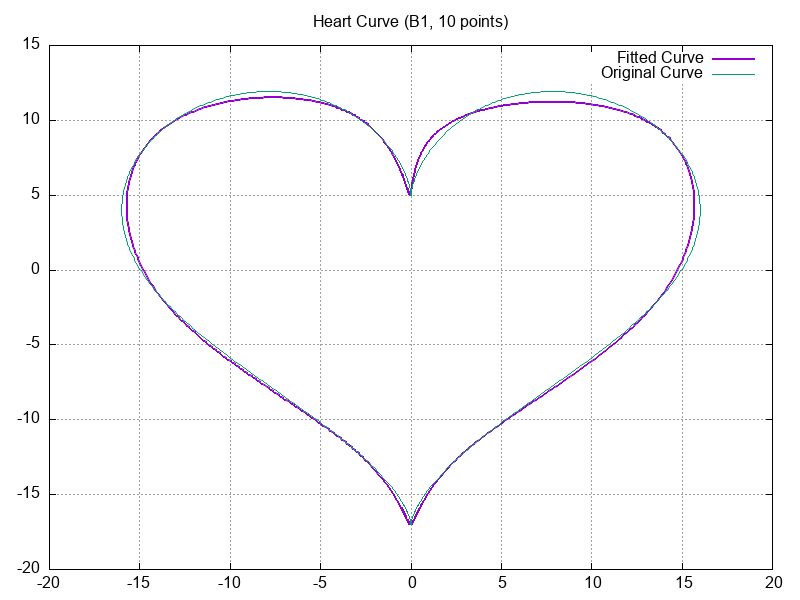
\includegraphics[width=0.48\textwidth]{../figure/B1heartspline_plot_10.png}
    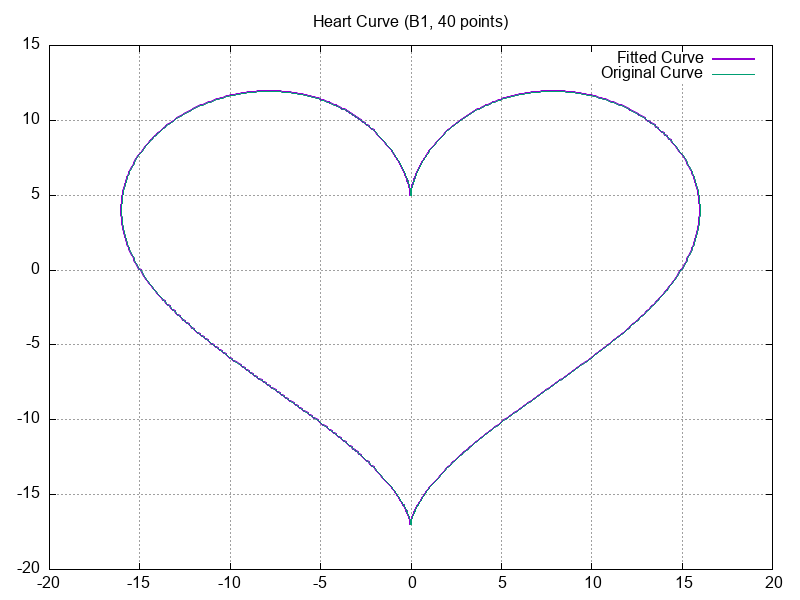
\includegraphics[width=0.48\textwidth]{../figure/B1heartspline_plot_40.png}
    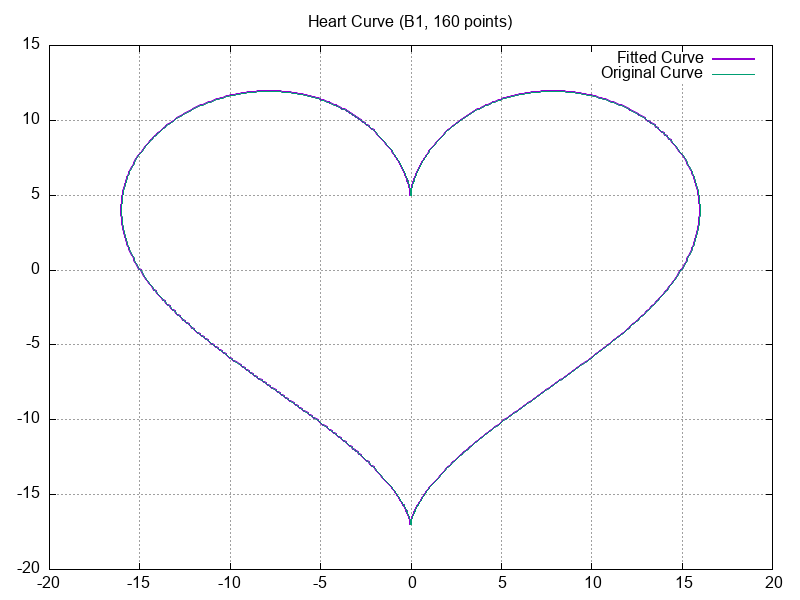
\includegraphics[width=0.48\textwidth]{../figure/B1heartspline_plot_160.png}
    \caption{Natural of Heart Curve, Node values 10, 40, 160}
\end{figure}

\begin{figure}[H]
    \centering
    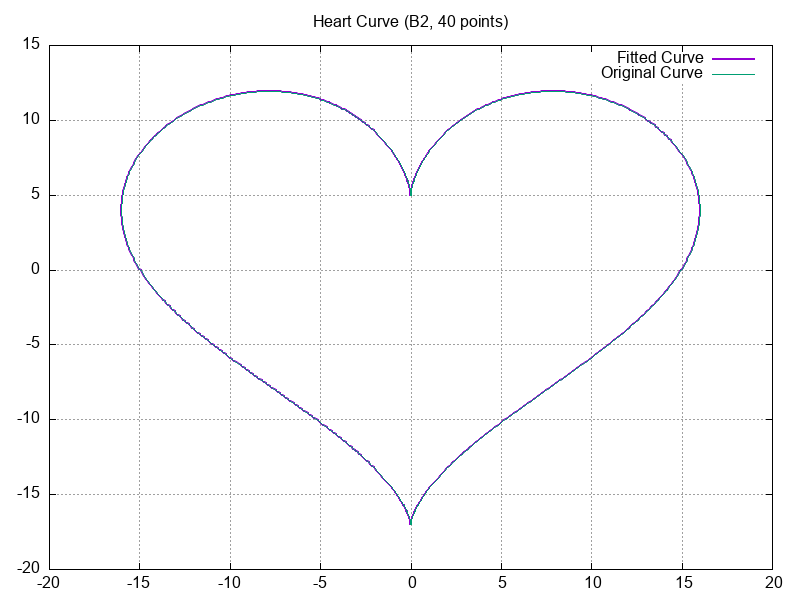
\includegraphics[width=0.48\textwidth]{../figure/B2heartspline_plot_40.png}
    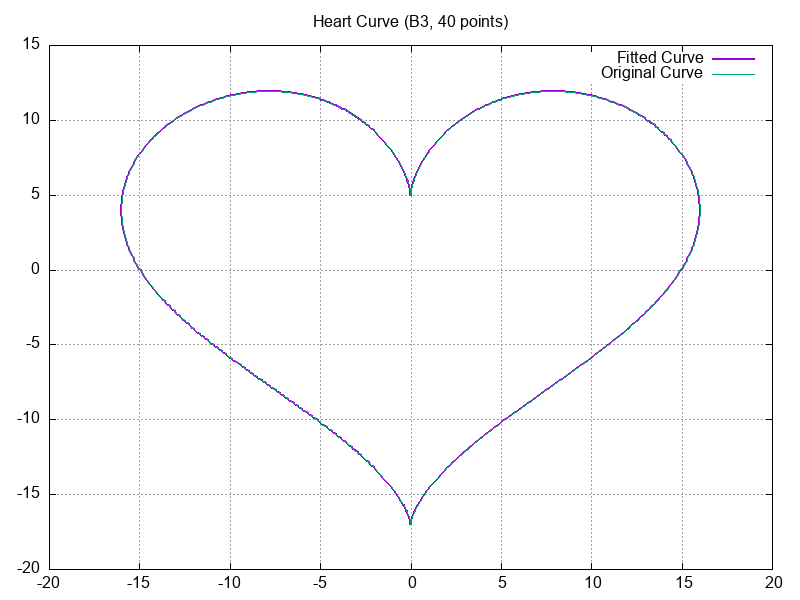
\includegraphics[width=0.48\textwidth]{../figure/B3heartspline_plot_40.png}
    \caption{Clamped and Periodic of Heart Curve, Node values 40}
\end{figure}

\begin{figure}[H]
    \centering
    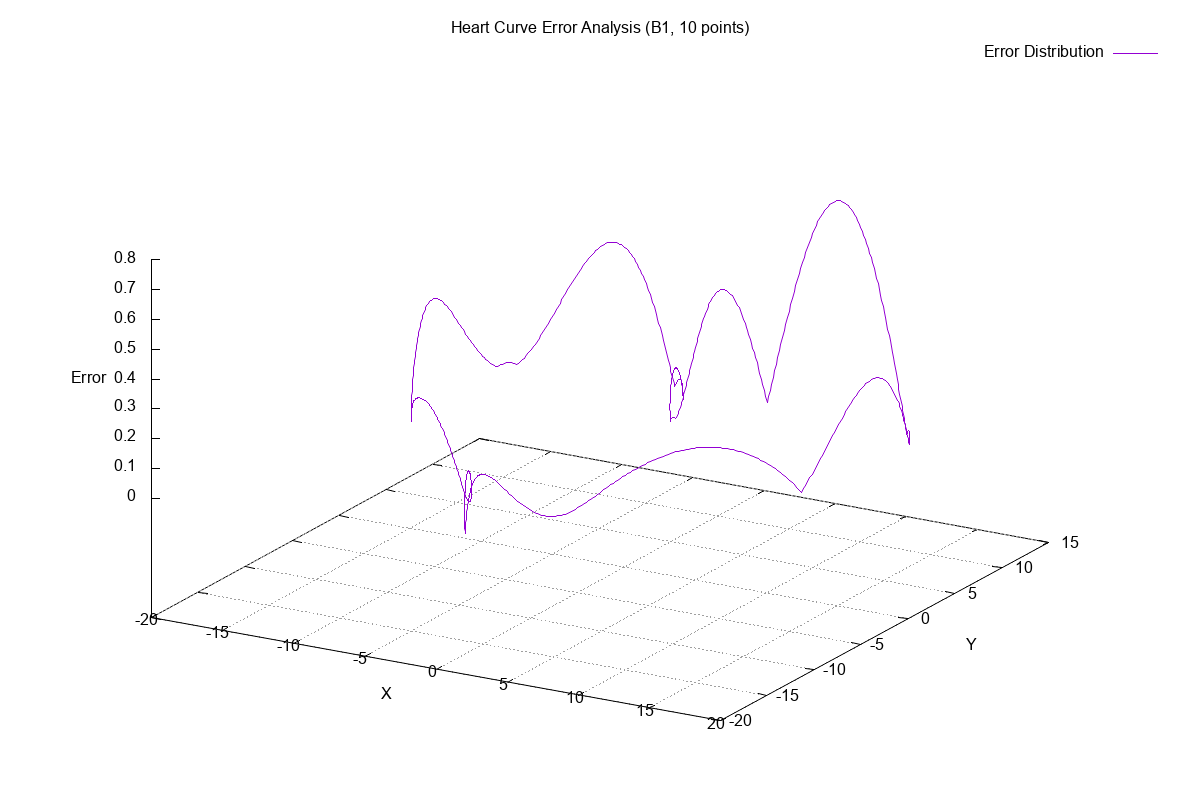
\includegraphics[width=0.48\textwidth]{../figure/B1heartspline_error3d_10.png}
    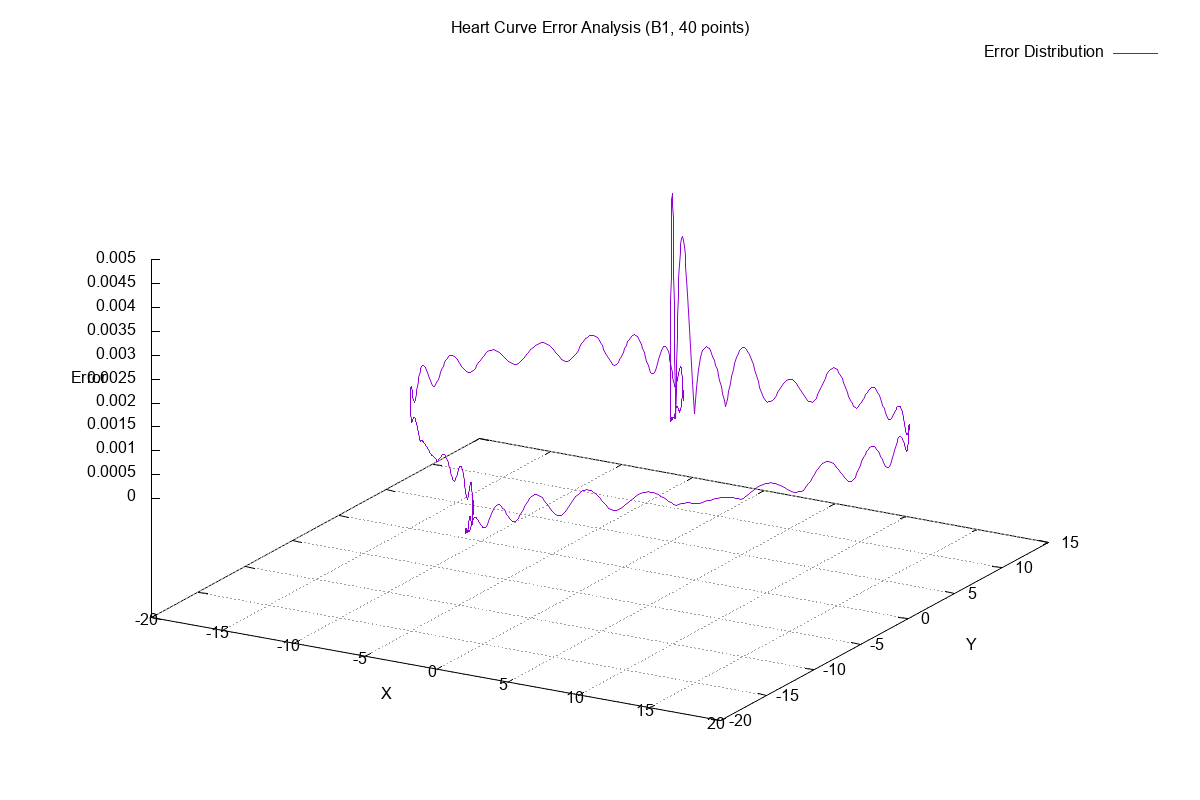
\includegraphics[width=0.48\textwidth]{../figure/B1heartspline_error3d_40.png}
    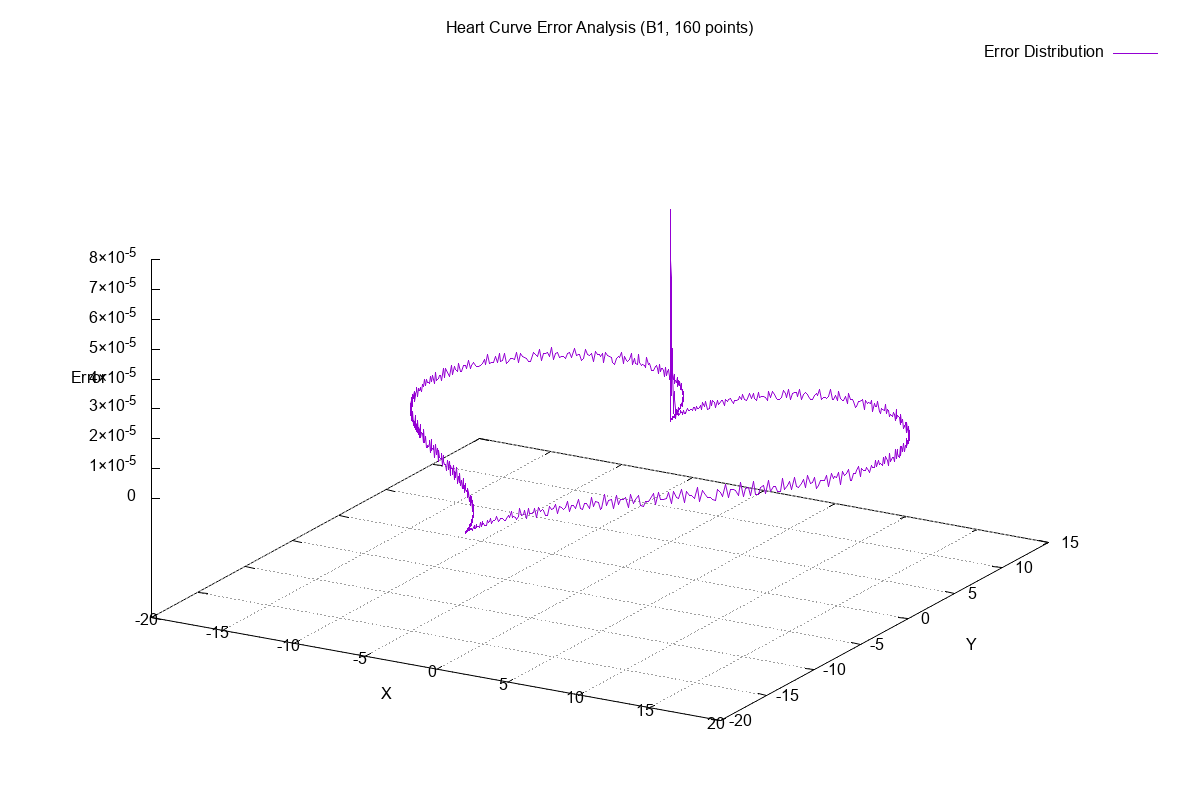
\includegraphics[width=0.48\textwidth]{../figure/B1heartspline_error3d_160.png}
    \caption{Natural Error of Heart Curve, Node values 10, 40, 160}
\end{figure}

\begin{enumerate}
    \item The error plots demonstrate the impact of the number of points on the accuracy of the B-spline interpolation. As the number of points increases, the error decreases significantly, indicating a more accurate interpolation.
    \item The relatively large error at the endpoint is due to the fact that the B-spline base does not completely cover the region.\
\end{enumerate}

For curve \(r_2\) (do not have periodic boundary conditions) and \(r_3\), we have:
\begin{figure}[H]
    \centering
    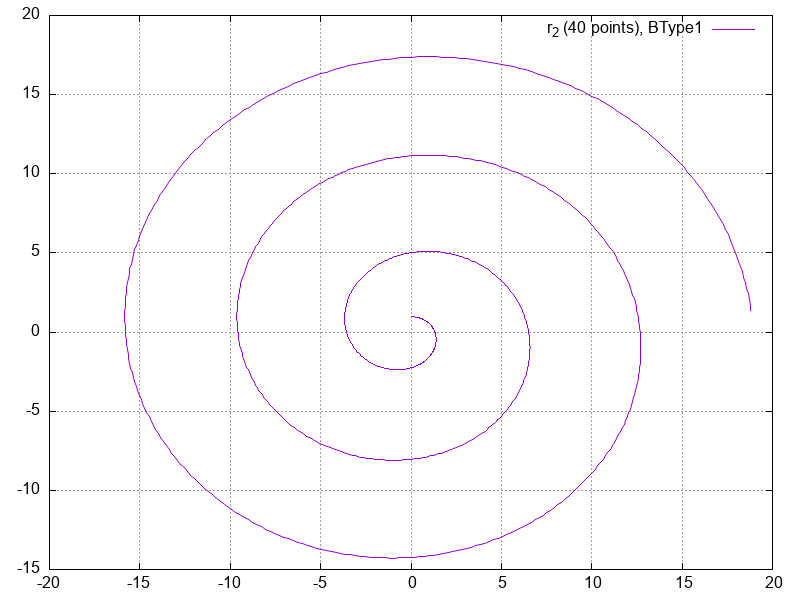
\includegraphics[width=0.48\textwidth]{../figure/B1r2spline_plot_40.png}
    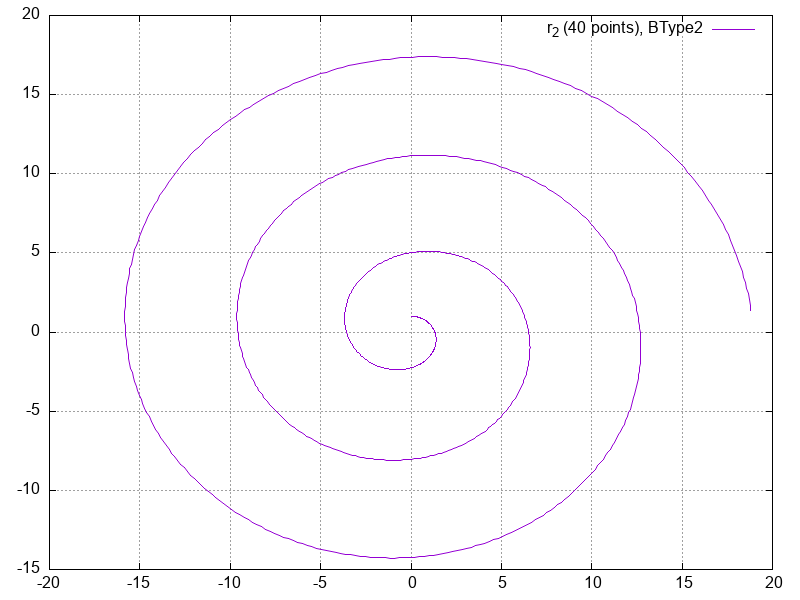
\includegraphics[width=0.48\textwidth]{../figure/B2r2spline_plot_40.png}
    \caption{Natural and Clamped of \(r_2\), Node values 40}
\end{figure}

\begin{figure}[H]
    \centering
    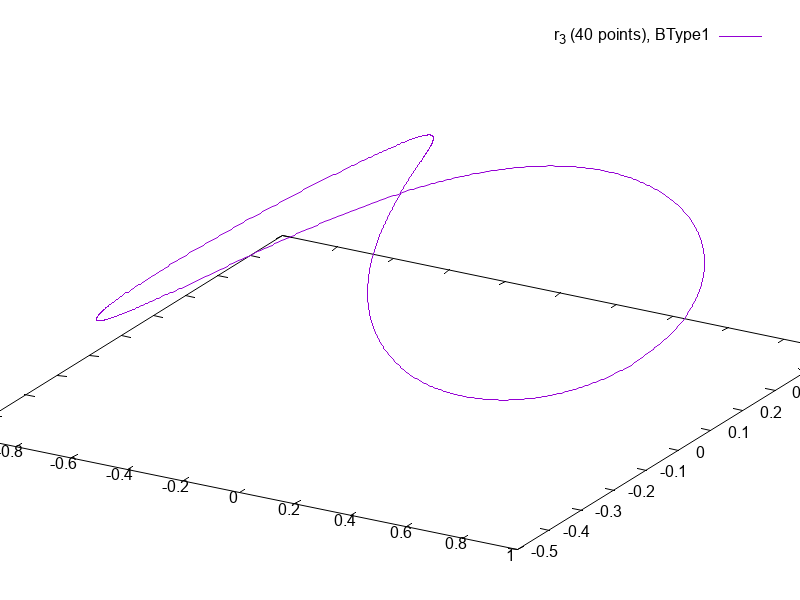
\includegraphics[width=0.48\textwidth]{../figure/B1r3spline_plot_40.png}
    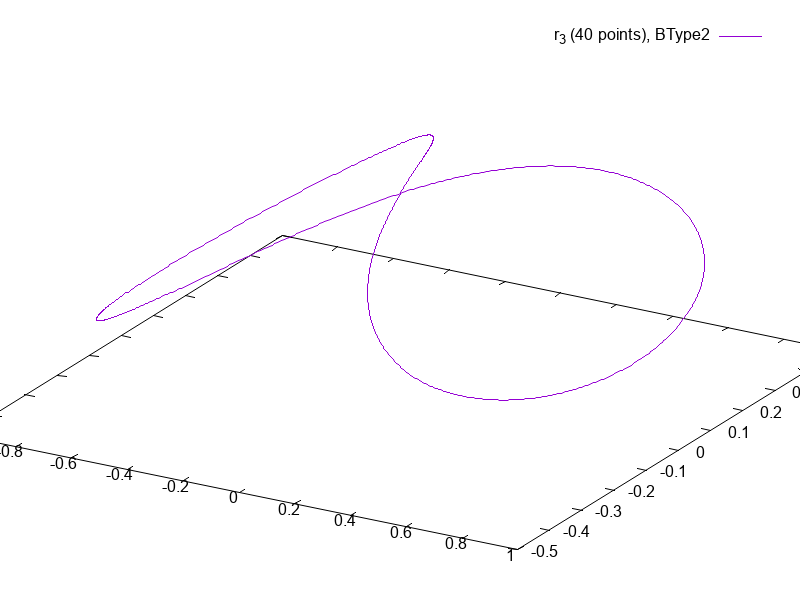
\includegraphics[width=0.48\textwidth]{../figure/B2r3spline_plot_40.png}
    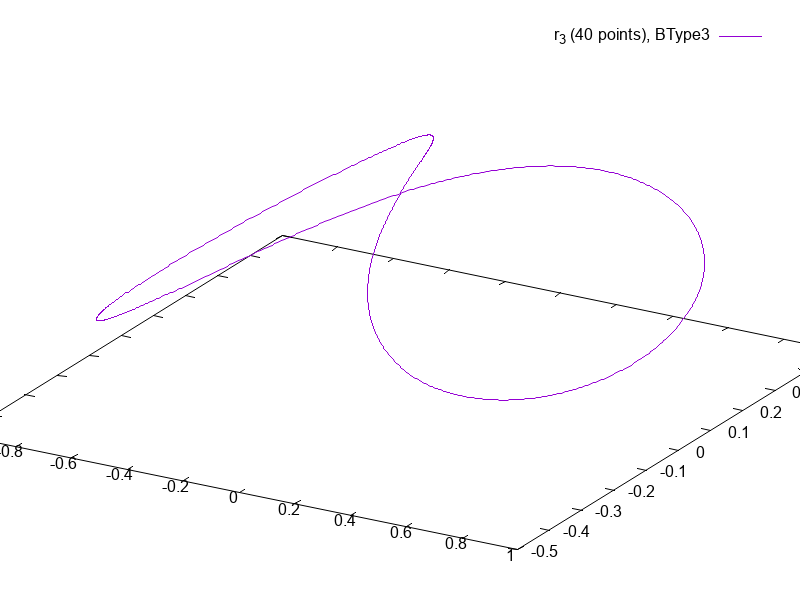
\includegraphics[width=0.48\textwidth]{../figure/B3r3spline_plot_40.png}
    \caption{Natural, Clamped and Periodic of \(r_3\), Node values 40}
\end{figure}

\subsubsection{Cumulative Chordal Length Method}
The \textit{cumulative chordal lengths} of a point sequence \((x_i)_{i=1}^N\) in \(\mathbb{R}^D\) form a sequence of \(N\) real numbers,
\[
t_i = 
\begin{cases} 
0, & \text{if } i = 1; \\
t_{i-1} + \|\mathbf{x}_i - \mathbf{x}_{i-1}\|_2, & \text{otherwise},
\end{cases}
\]
where \(\|\cdot\|_2\) denotes the Euclidean 2-norm.\par
So we get the new parameter and use the new parameter for B-spline curve fitting. Here, we show the curve fitting results of the three curves above (Heart Curve, \(r_2\) and \(r_3\) with Natural boundary conditions of node values 40; Error of Heart Curve with Natural boundary conditions of node values 40;) :

\begin{figure}[H]
    \centering
    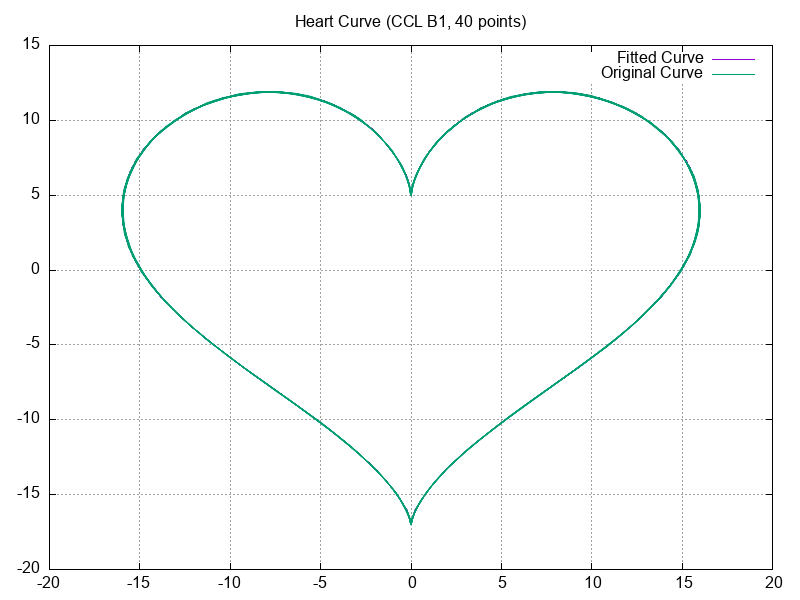
\includegraphics[width=0.48\textwidth]{../figure/B1CCLheartspline_plot_40.png}
    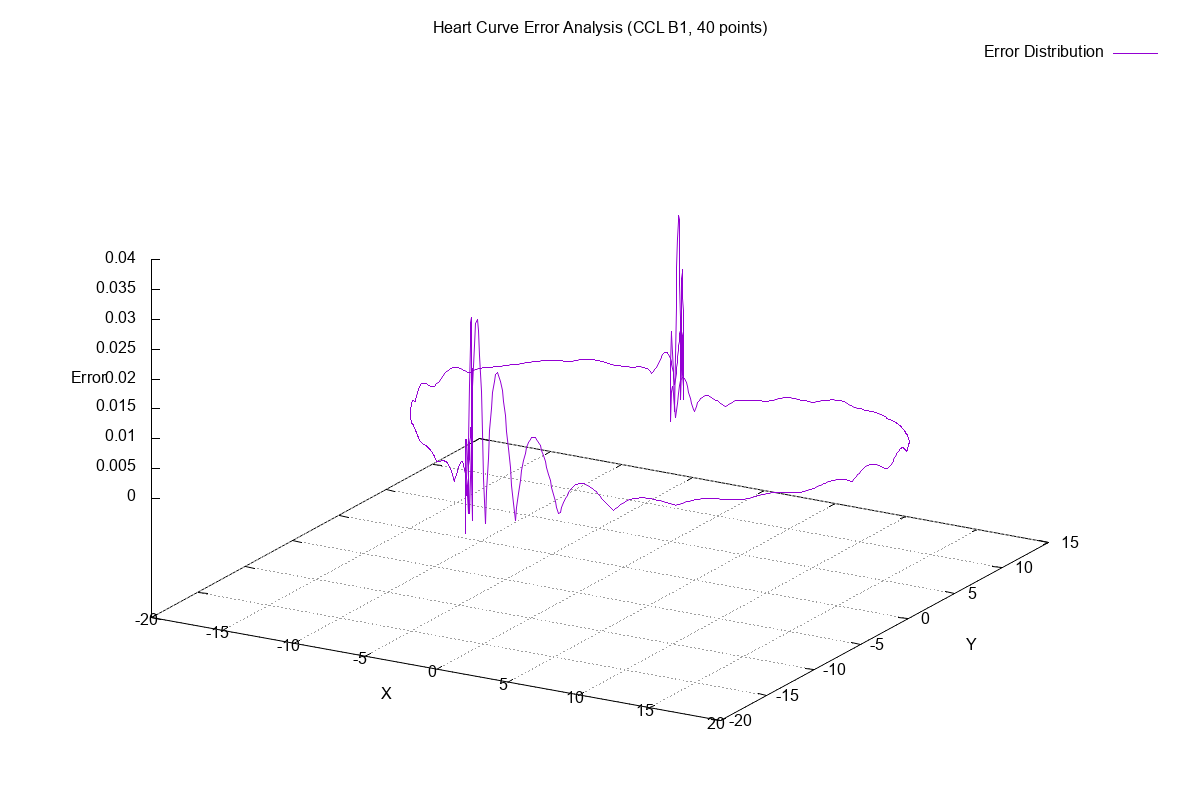
\includegraphics[width=0.48\textwidth]{../figure/B1CCLheartspline_error3d_40.png}
    \caption{Natural of Heart Curve, Node values 40}
\end{figure}

\begin{figure}[H]
    \centering
    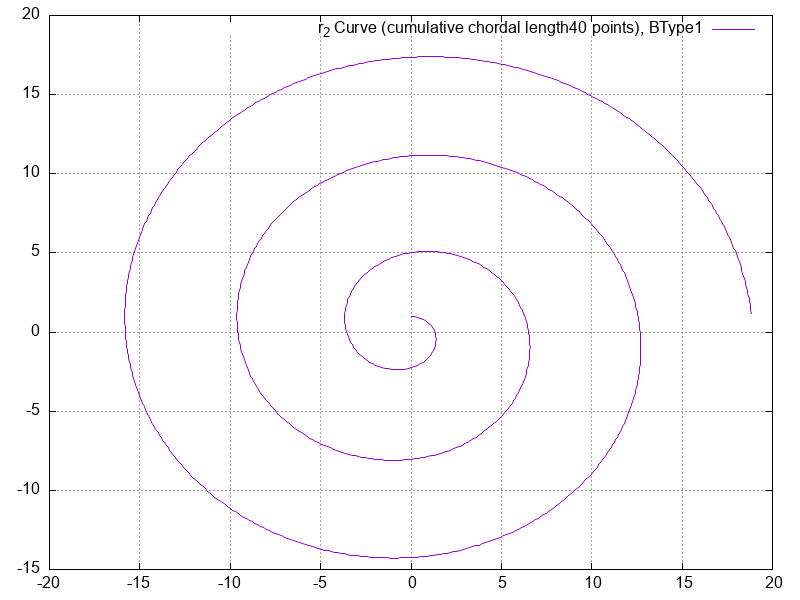
\includegraphics[width=0.48\textwidth]{../figure/B1CCLr2spline_plot_40.png}
    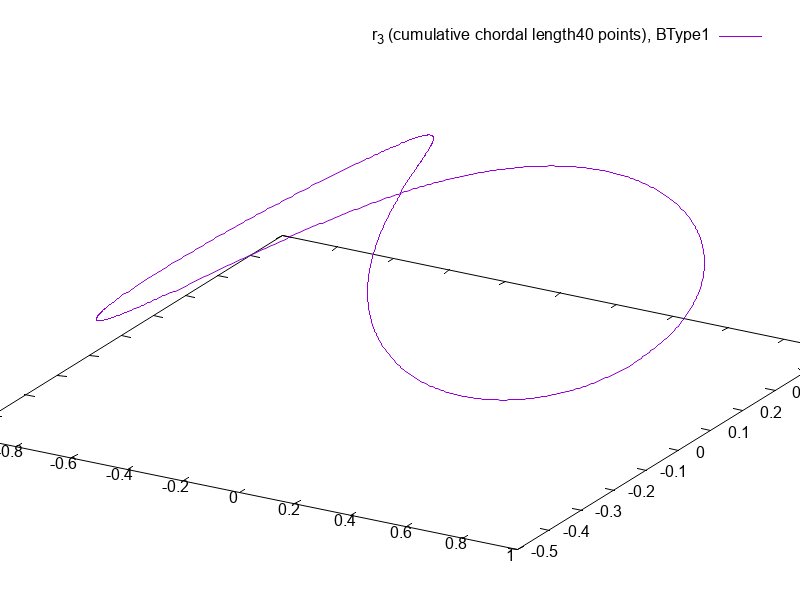
\includegraphics[width=0.48\textwidth]{../figure/B1CCLr3spline_plot_40.png}
    \caption{Natural of \(r_2\) and \(r_3\), Node values 40}
\end{figure}

\subsubsection{Compare the Two Parameterizations}
Output by the program, we have:
\begin{table}[H]
\centering
\begin{tabular}{|c|c|c|}
\hline
Spline Type & Maximum Error & Average Error \\ \hline
Natural(Uniform) & 0.00477674 & 0.000369366 \\ 
Clamped(Uniform) & 0.000714064 & 0.000216572  \\ 
Periodic(Uniform) & 0.000714051 & 0.000216687  \\ \hline
Natural(CCL) & 0.0354496 & 0.0032255  \\ 
Clamped(CCL) & 0.0354496 & 0.00379937  \\ 
Periodic(CCL) & 0.0354496 & 0.00397928  \\ \hline
\end{tabular}
\caption{Error Analysis for Different Numbers of Nodes}
\label{tab:error_analysis}
\end{table}
By comparing the maximum and average errors of the heart curve at N=40 under the three boundary conditions, we can observe the CCL parameterization results in higher errors compared to the Uniform parameterization.\par
When the data points change sharply (two cusps of the heart curve), the curves parameterized by the cumulative chord length may perform poorly in smoothness. This is because when dealing with fast-changing data points, cumulative chord length parameterization may not transition smoothly when nodes happen to span fast-changing regions, resulting in unnatural curves or fluctuations in the curves of those regions.


\subsection{Curve-fitting on the Unit Ball}
See \texttt{CurveonBall.cpp} for the test code.\par
Here, we use the curve \(r_3\) above as the test case.
\subsubsection{Methodology}
The implementation involves the following steps:
\begin{enumerate}
    \item Generation of parameter points on the sphere.
    \item Application of the Riemann mapping to transform the spherical curve into a planar curve.
    \item Construction of cubic B-splines for the transformed curve.
    \item Inversion of the Riemann mapping to map the planar spline back onto the sphere.
\end{enumerate}

\subsubsection{Riemann Mapping and Its Inverse}
The Riemann ball realizes a mapping: \(\partial B \backslash N \rightarrow \mathbb{R}^2\), \(N = P(\infty)\).\par

\begin{figure}[H]
    \centering
    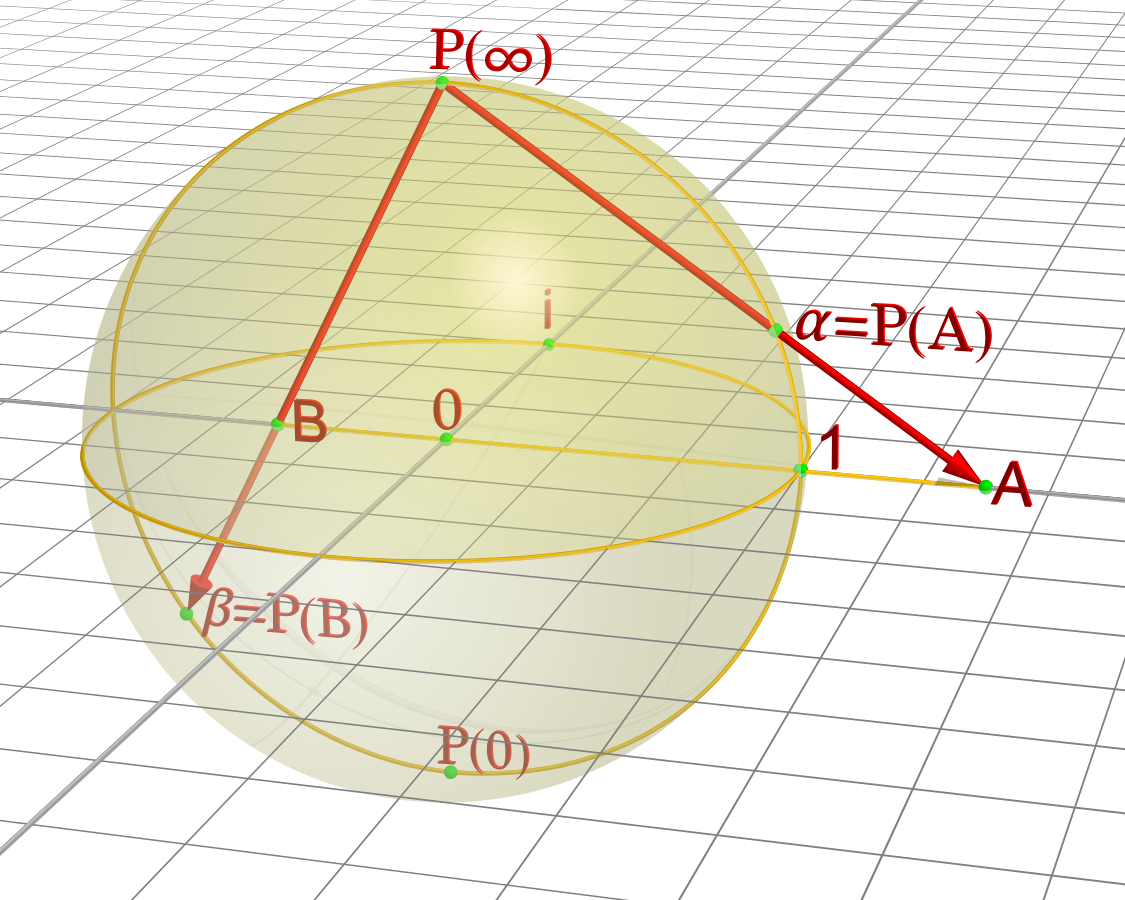
\includegraphics[width=0.8\textwidth]{../figure/RiemannBall.png}
    \caption{Riemann Mapping.}
    \label{fig:Riemann}
\end{figure}

The Riemann mapping is defined as:
\[
x_{\text{Plane}} = \frac{0.5x_{\text{Ball}}}{1 - 0.5(z_{\text{Ball}} + 1)}, \quad
y_{\text{Plane}} = \frac{0.5y_{\text{Ball}}}{1 - 0.5(z_{\text{Ball}} + 1)}, \quad
\]
where \( t \) is the parameter along the curve.

The inverse Riemann mapping is given by:
\begin{align*}
    &x_{\text{Ball}} = \frac{2x_{\text{Plane}}}{x_{\text{Plane}}^2 + y_{\text{Plane}}^2 + 1}, \\
    &y_{\text{Ball}} = \frac{2y_{\text{Plane}}}{x_{\text{Plane}}^2 + y_{\text{Plane}}^2 + 1}, \\
    &z_{\text{Ball}} = \frac{2(x_{\text{Plane}}^2 + y_{\text{Plane}}^2)}{x_{\text{Plane}}^2 + y_{\text{Plane}}^2 + 1} - 1  
\end{align*}

\subsubsection{Results}
Since the \(N\) point is not defined, we do mirror symmetry with respect to the \(XY\) plane for \(r_3\).\par
The test results are visualized in the provided images, showing the spline fitting on the Riemann sphere for different numbers of points (10, 40, 160). The spline closely follows the original curve, demonstrating the effectiveness of the method.

\begin{figure}[H]
    \centering
    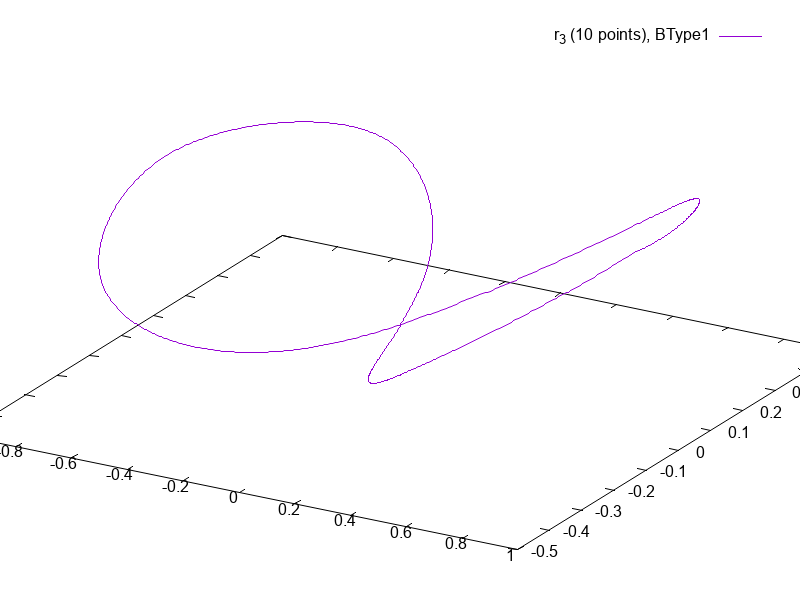
\includegraphics[width=0.3\textwidth]{../figure/B1r3spline_ball_10.png}
    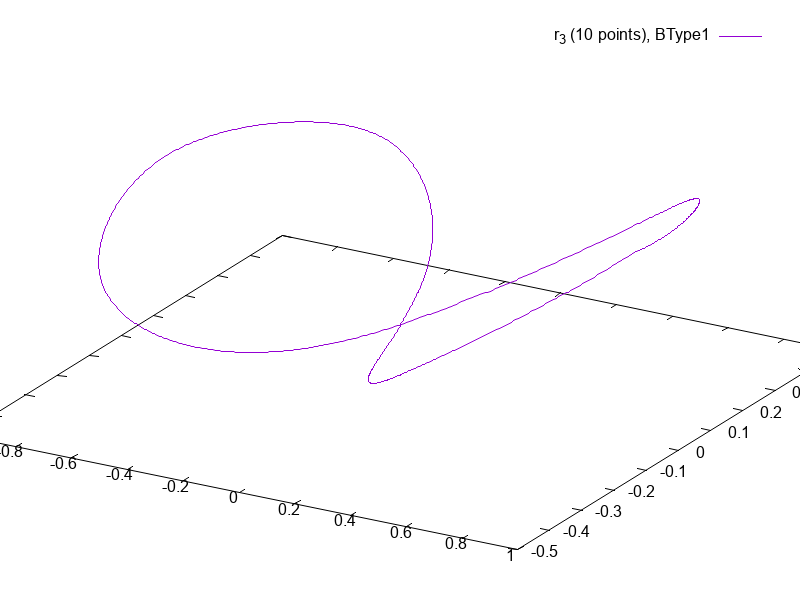
\includegraphics[width=0.3\textwidth]{../figure/B1r3spline_ball_10.png}
    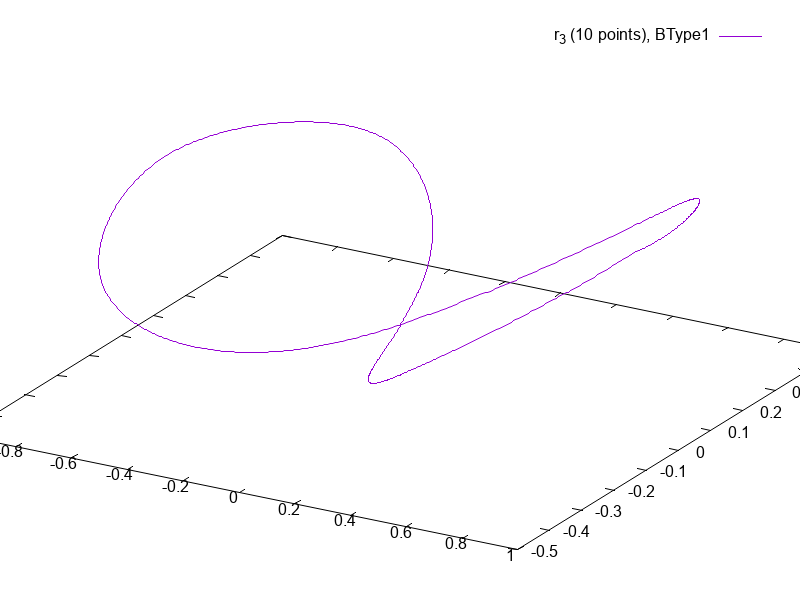
\includegraphics[width=0.3\textwidth]{../figure/B1r3spline_ball_10.png}
    \caption{Spline fitting on ball with 10, 40 and 160 points.}
    \label{fig:ball}
\end{figure}

\subsubsection{Discussion}
The results indicate that the spline fitting on the Riemann sphere is robust and accurate, especially as the number of points increases. The use of the Riemann mapping allows for straightforward spline construction in a planar space, which is computationally more manageable.


\section{Compare pp-Form with B-Form}
See \texttt{compareppwithBcurve.cpp} for the test code.\par
Here, we interpolate the heart-shaped curve with three boundary conditions, pp-Form and B-Form, respectively, to compare the errors of the two fitted curves (number of nodes \(N=40\)).
\subsection{Methodology}
The test was implemented in the following steps:
\begin{enumerate}
    \item Generation of parameter points for the heart curve.
    \item Calculation of x and y points for the heart curve.
    \item Creation of Cubic pp-Splines and Cubic B-Splines for x(t) and y(t) with the same set of control points and boundary conditions.
    \item Calculation of the error between the pp-Spline and B-Spline curves at a higher resolution.
    \item Generation of 3D error distribution plots using Gnuplot.
\end{enumerate}

\subsection{Results}
The test was conducted for three different spline types (1-Natural, 2-Clamped, 3- Periodic) with 40 control points each. The following 3D error distribution plots were generated:

\begin{figure}[H]
    \centering
    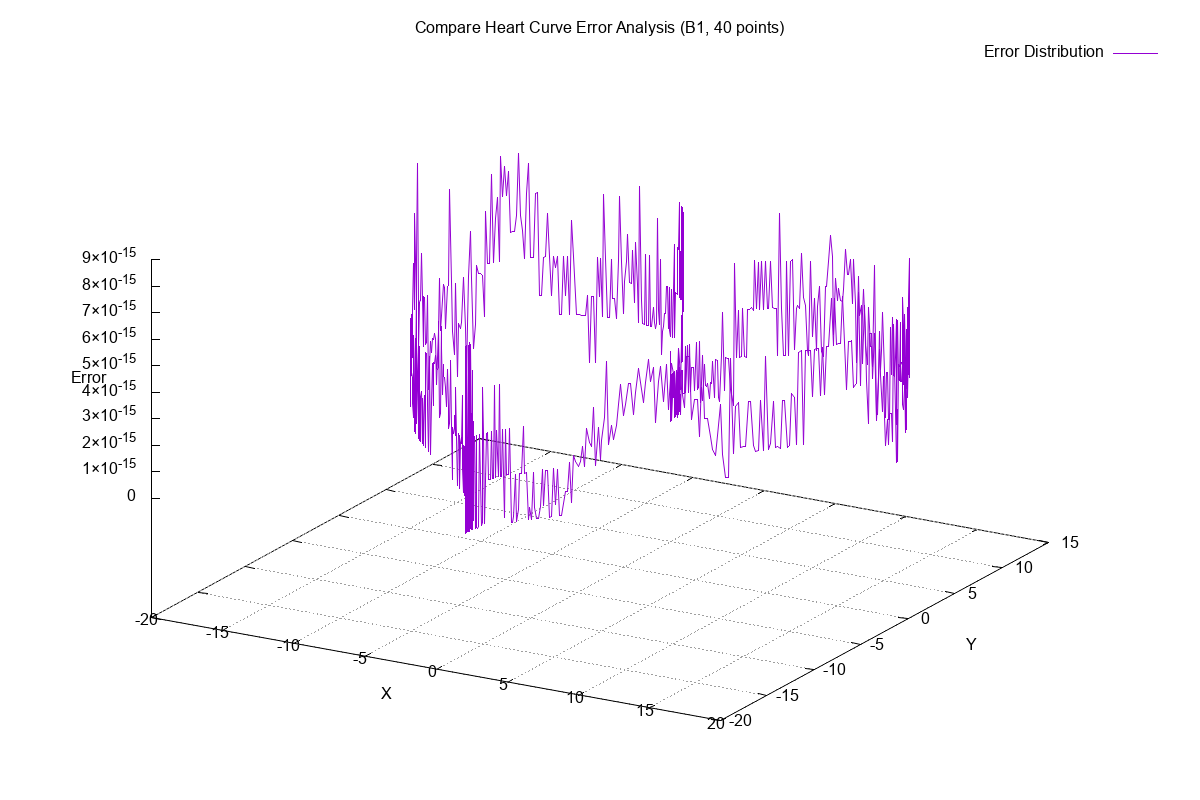
\includegraphics[width=0.5\textwidth]{../figure/compare_1heartspline_error3d_40.png}
    \caption{Error distribution for Natural boundary conditions.}
    \label{fig:b1_error}
\end{figure}

\begin{figure}[H]
    \centering
    \includegraphics[width=0.5\textwidth]{../figure/compare_2heartspline_error3d_40.png}
    \caption{Error distribution for Clamped boundary conditions.}
    \label{fig:b2_error}
\end{figure}

\begin{figure}[H]
    \centering
    \includegraphics[width=0.5\textwidth]{../figure/compare_3heartspline_error3d_40.png}
    \caption{Error distribution for Periodic boundary conditions.}
    \label{fig:b3_error}
\end{figure}

\subsection{Discussion}
The error distribution plots indicate that the pp-Form and B-Spline methods produce very similar results, with the error being on the order of $10^{-15}$ to $10^{-14}$. This level of error is close to machine error, suggesting that both methods are equivalent in this context.


\section{More Function Sample Tests}
\subsection{\(sin \pi x, \quad x\in [-1, 1]\)}
See the results in part \textbf{Test Linear pp-Form} and \textbf{Test Cubic pp-Form}.

\subsection{\( f(x) = \frac{1}{e^{x^2}}, \quad x\in [-3, 3] \)}
See the result in part \textbf{Test Degree 5 pp-Spline}.

\subsection{Other Tests of Curve-fitting on the Unit Ball}
\subsubsection{\(r_4\)}
The parametric equation for \(r_4\) is:
\begin{align*}
&x = sin(cos(2t))cos(t),\\
&y = sin(cos(2t))sin(t),\\
&z = -cos(cos(2t)),\\
&where \quad t \in [0, 2\pi].    
\end{align*}
The results are shown below:
\begin{figure}[H]
    \centering
    \includegraphics[width=0.3\textwidth]{../figure/B1r4spline_ball_10.png}
    \includegraphics[width=0.3\textwidth]{../figure/B1r4spline_ball_40.png}
    \includegraphics[width=0.3\textwidth]{../figure/B1r4spline_ball_160.png}
    \caption{Spline fitting of \(r_4\) on ball with 10, 40 and 160 points.}
    \label{fig:ball2}
\end{figure}

\subsubsection{\(r_5\)}
The parametric equation for \(r_5\) is:
\begin{align*}
&x = sin(cos(t) + 0.5)cos(sin(2t)),\\
&y = sin(cos(t) + 0.5)sin(sin(2t)),\\
&z = -cos(cos(t) + 0.5),\\
&where \quad t \in [0, 2\pi].    
\end{align*}
The results are shown below:
\begin{figure}[H]
    \centering
    \includegraphics[width=0.3\textwidth]{../figure/B1r5spline_ball_10.png}
    \includegraphics[width=0.3\textwidth]{../figure/B1r5spline_ball_40.png}
    \includegraphics[width=0.3\textwidth]{../figure/B1r5spline_ball_160.png}
    \caption{Spline fitting of \(r_5\) on ball with 10, 40 and 160 points.}
    \label{fig:ball3}
\end{figure}


\section{Problem F}
See \texttt{ProblemF2.cpp, ProblemF2.cpp} for the test code.
\subsection{Results}

The test generated the following plots for \( n=1 \) and \( n=2 \):

\begin{figure}[H]
    \centering
    \includegraphics[width=\textwidth]{../figure/basis_functions_n1.png}
    \caption{Plots for \( n=1 \): Truncated power functions and first and second divided differences.}
    \label{fig:n1_plots}
\end{figure}

\begin{figure}[H]
    \centering
    \includegraphics[width=\textwidth]{../figure/basis_functions_n2.png}
    \caption{Plots for \( n=2 \): Truncated power functions and first, second, and third divided differences.}
    \label{fig:n2_plots}
\end{figure}

As shown in the figure, we verify that \(n=1\) and \(n=2\) satisfy:\par
For any \( n \in \mathbb{N} \),
\[ B_i^n(x) = (t_{i+n} - t_{i-1}) \cdot [t_{i-1}, \ldots, t_{i+n}] (t - x)_+^n. \]


\section{Self-Intersection Detection}
See \texttt{intersection.cpp} for the test code.\par
The program employs a parametric curve definition and a distance calculation algorithm to identify potential intersections.
\subsection{Methodology}
The program operates through the following steps:
\begin{enumerate}
    \item Generation of curve points using a parametric equation.
    \item Calculation of the distance between two line segments in 3D space.
    \item Detection of self-intersection by comparing segment distances against a threshold.
\end{enumerate}

\subsubsection{Curve Definition}
Here we use the \(r_3\) mentioned above as the test curve. The curve is parametrically defined as:
\[ x = \sin(\cos(t)) \cos(\sin(t)), \]
\[ y = \sin(\cos(t)) \sin(\sin(t)), \]
\[ z = \cos(\cos(t)), \]
where \( t \) ranges from \( 0 \) to \( 2\pi \).

\subsubsection{Distance Calculation}
The distance between two line segments \( p1p2 \) and \( p3p4 \) is calculated using the algorithm outlined below:
\begin{enumerate}
    \item Compute vectors \( \mathbf{u} = p2 - p1 \), \( \mathbf{v} = p4 - p3 \), and \( \mathbf{w} = p3 - p1 \).
    \item Calculate dot products \( a = \mathbf{u} \cdot \mathbf{u} \), \( b = \mathbf{u} \cdot \mathbf{v} \), and \( c = \mathbf{v} \cdot \mathbf{v} \).
    \item Compute the cross product \( \mathbf{dP} = \mathbf{w} - (\mathbf{u} \cdot \mathbf{w} / a) \mathbf{u} - (\mathbf{v} \cdot \mathbf{w} / c) \mathbf{v} \).
    \item The distance is then \( \sqrt{\mathbf{dP} \cdot \mathbf{dP}} \).
\end{enumerate}

\subsubsection{Self-Intersection Detection}
The program checks for self-intersection by iterating through pairs of curve segments. For each pair, it:
\begin{enumerate}
    \item Computes the distance between the segments using the line segment distance function.
    \item Compares this distance to a predefined threshold. If the distance is less than the threshold, the curve is considered to self-intersect at that point.
\end{enumerate}

\subsection{Results}
The program execution resulted in the detection of a self-intersection within the curve. With the default parameters set (1000 samples, a threshold of \(1 \times 10^{-5}\), and a minimum segment distance of 10), the program successfully identified that at least one pair of line segments had a distance less than the predefined threshold, indicating that the curve intersects itself at some point.

\subsection{Discussion}
The algorithm effectively identifies potential self-intersections by calculating the minimum distance between all possible pairs of line segments. The use of a threshold allows for flexibility in determining what constitutes an intersection based on the application's precision requirements.


\end{document}